%\documentclass[a4paper,conference]{IEEEtran}
%\documentclass[a4paper,10pt,conference]{ieeeconf}
%\documentclass[usletter, 10pt, conference]{ieeeconf}      % Use this line for a4 paper
%\IEEEoverridecommandlockouts                              % This command is only needed if 
%\overrideIEEEmargins                                      % Needed to meet printer requirements.

\documentclass{llncs}

\usepackage{graphicx}
\usepackage{booktabs}
\usepackage{amsmath}
\usepackage[ruled,lined]{algorithm2e}
\usepackage{multirow}
\usepackage[bookmarks=false]{hyperref}
\pdfminorversion=4

\newcommand{\red}[1]{\textcolor{red}{#1}}

\hypersetup{colorlinks=true,linkcolor=black,citecolor=black}

\SetKwInput{KwData}{Global params.}

\title{
    Analysis of protein tunnel traversability for flexible ligands
}

\author{Vojt\v ech Von\' asek\inst{1} \and Barbora Kozl\'\i kov\'a\inst{2} \and Adam Jur\v{c}\'\i k\inst{2} \and Martin Saska\inst{1}}
\institute{
Faculty of Electrical Engineering,  
Czech Technical University in Prague, 
Technick\'a 2, 166 27, Prague 6, Czech Republic
\email{vonasek@labe.felk.cvut.cz}
\and
Faculty of Informatics,  
Masaryk University, 
Botanick\'a 68a, 602 00 Brno,
}


%This work was supported by Grant Agency of the Czech Technical University in Prague, grant No. SGS15/157/OHK3/2T/13.
%Access to computing and storage facilities owned by parties and projects contributing to the National Grid Infrastructure MetaCentrum, provided under the programme "Projects of Large Infrastructure for Research, Development, and Innovations" (LM2010005), is greatly appreciated.
%vonasek@labe.felk.cvut.cz.

\def\qrand{q_{rand}}
\def\qstart{q_{start}}
\def\qinit{\qstart}
\def\qnear{q_{near}}
\def\qnew{q_{new}}
\def\C{\mathcal{C}}
\def\T{\mathcal{T}}
\def\CF{\mathcal{C}_{free}}
\def\Imax{I_{max}} %max number of iterations of RRT-based planners

\def\dist{\mathrm{dist}}
\def\dists{\mathrm{dist}_{\mathrm{s}}}

\SetKw{return}{return}

\def\VV{V_{vor}}
\def\VVA{V_{vor}^{act}}
\def\da{d_{high}}
\def\db{d_{low}}


\def\TA{$A_1$}
\def\TB{$A_2$}
\def\TC{$A_3$}

\def\probe{r_{\mathrm{probe}}}
\def\Sprobe{S_{\mathrm{probe}}}

\def\gprobe{r_{\mathrm{out}}}
\def\Sgprobe{S_{\mathrm{out}}}


\def\CG{\mathcal{C}_{goal}}
\def\SB{\mathbf{S}_{blocking}}
\def\SS{\mathbf{S}}

\def\RRTTD{RRT$_{\mathrm{td}}$}
\def\RRTN{RRT$_{\mathrm{n}}$}
\def\ths{d_\mathrm{surf}}

%spacing for algorithm environment. 1.0 mean normal spacing
\def\gb{p_{c}}

\begin{document}

\maketitle
%\frontmatter          % for the preliminaries


\begin{abstract}
Proteins are involved in many biochemical processes.
%Behavior and properties of proteins as well as other bio-macromolecules are influenced by internal void space such as tunnels or cavities.
Behavior of proteins is influenced by internal void space such as tunnels or cavities.
Tunnels are paths leading from an active site inside the protein to its surface.
Knowledge about tunnels and their evolution in time provides an insight into protein properties
(e.g., stability).
Sampling-based motion planning methods like Rapidly Exploring Random Tree (RRT) can be used to find the tunnels by
sampling the corresponding configuration space.
The main advantage of these methods is that they can be easily adapted to consider protein dynamics.
%i.e., they can find tunnels in proteins moving in time.
However, the inner void space of proteins is  very limited, 
    which may decrease ability of RRT to find a solution due to the narrow passage problem.
In this paper, we propose to generate the random samples using Voronoi Diagram of the atoms.
A subset of Voronoi vertices is dynamically maintained to support generation of samples in promising regions inside the protein.

%VD provides initial information about protein void space, which helps to sample the corresponding configuration space.

%While VD of the protein atoms can be easily computed, the RRT is used to cope with the protein dynamics<F12>
%While the VD provides
%Random samples are generated around a subset of vertices of VD 

%and modifications to support searching of multiple tunnels in each frame.
%In the comparison to existing literature on sampling using Voronoi diagrams, the proposed technique supports finding of multiple
%tunnels even in dynamic proteins.
%The proposed approach is compared to CAVER 3.0, one of the widely used freely available tools for protein analysis.
%In this paper, we propose a novel sampling technique for the purpose of tunnel detection in protein structures.
%The protein void space can be search using sampling-based
%The classical approach to find tunnels in protein structures is based on Voronoi diagrams (VD), which is suitable
%for tunnel detection in a single snapshot of protein's dynamics.
%To consider protein dynamics, that is represented by a sequence of protein snapshots, correspondences between
%VD in these snapshots need to be found, which is time and memory consuming.
%An alternative approach is to employ motion planning methods to detect the tunnels.
%However, VD-based computation can be time consuming when protein dynamics needs to be considered, as it
%requires to find correspondences between VD in a sequence of frames of protein dynamics.
%The performance of VD-based tunnel detection is decreased in the case of dynamic proteins, which requires
%to find correspondences between VD in frames of molecular dynamics.
%In order to apply the VD-based approach for dynamic proteins,
%Available methods for tunnel detection assume static proteins, which allows us to detect tunnels using Voronoi Diagrams.
%Tunnels in static proteins however  provide only a  rough idea about protein behavior.
%Tunnels in real proteins are however influenced by dynamics of the protein.
%In this paper, we describe tunnel detection using Rapidly Exploring Random Tree (RRT).
%The method builds a single configuration tree describing free space of the protein. 
%A crucial part of this novel approach is the sampling of the internal void space of the protein.
%The nodes of the tree are pruned according to protein dynamics.
\end{abstract}

\section{Introduction}
%{\color{red}Co bys rikala na to dat na 1. stranku nejaky obrazek tunelu?}

Protein structures are essential components of all living organisms.
Proper understanding of their structure and function is important in many fields, including drug design, agriculture, cosmetics, etc.
Although this knowledge is still very hard to reveal, several protein structures have been already investigated in sufficient detail. % which led to their better understanding. 
Such investigation can incorporate computational methods which help to analyze the geometry of protein structure,  its shape, surface area, and inner void space. 
%These parameters then suggest and influence protein behavior, namely its reactivity with other molecules.
%consists of the analysis of protein structure, its shape, surface area, and inner void space. 
%These parameters influence namely the protein reactivity. % which is one of the most often studied behavior of the protein.


%Proteins interact with other molecules (small ligands, ribonucleic acid chains, other proteins, etc.) which can lead to changes in properties of the protein or the interacting molecule.
%Thanks to protein interaction with other molecules (small ligands, ribonucleic acid chains, other proteins, etc.), 
% we are able to change the properties of the protein or the interacting molecule. 
 For example, one task in protein engineering is to change selected properties of a protein, e.g. its stability under different outer conditions~\cite{Koudelakova2013} or activity of the protein towards the other molecules~\cite{Pavlova2009}.
%This is reached by studying so called tunnels in proteins which can serve as the transportation paths for the ligand from the outside environment to the active site or vice versa.
%For example, typical task in protein engineering is to change selected properties of a protein, e.g. its stability under different outer conditions [11] or activity of the protein towards other molecules [16]. 
This can be achieved by detecting and studying so called tunnels in proteins which can serve as the transportation paths for the 
ligand from the outside environment to the active site or vice versa. 
The active site is a specific site, usually deeply buried inside the protein, 
    where the chemical reaction between the protein and ligand can undergo. 
The importance of tunnels can be demonstrated on the study where mutations of amino acids located directly around the tunnel substantially improved the structural and kinetic stability of the studied protein, while
surface mutations almost did not contribute to the stabilization~\cite{Koudelakova2013}.

%For example, one task in protein engineering is to change selected properties of a protein, e.g. its stability under different outer conditions~\cite{Koudelakova2013} or activity of the protein towards the other molecules~\cite{Pavlova2009}.
%This is reached by studying so called tunnels in proteins which can serve as the transportation paths for the ligand from the outside environment to the active site or vice versa.
%The active site is a specific site, usually deeply buried inside the protein, where the chemical reaction between the protein and ligand can undergo.
%Since the importance of the presence of tunnels in proteins was revealed, the researchers started to study them intensively.
%Koudel\'{a}kov\'{a} et al.~\cite{Koudelakova2013} show that mutations of amino acids located directly around the tunnel improved the structural and kinetic stability of the studied protein substantially, while the surface mutations almost did not contribute to protein stabilization.
%The importance of tunnel can be demonstrated on an example, 
% where mutations of amino acids located directly around the tunnel improved the structural 
%and kinetic stability of the studied protein substantially, while surface mutations almost did not contribute to
%the protein stabilization~\cite{Koudelakova2013}.

%On the other hand, surface mutations almost did not contribute to protein stabilization~\cite{Koudelakova2013}.


%The task of tunnel detection is to find a collision-free path leading from an active site inside the protein to its surface.
%As not all paths are biochemically relevant, only paths with a given minimal bottleneck have to be reported (the bottleneck is
%the radius of the smallest sphere that can traverse the whole tunnel) 

Generally, the task of tunnel detection is to find a collision-free path leading from the active site to the protein's surface. 
The path is usually searched for a spherical probe of a given radius, which serves as a proxy geometry for a ligand. 
An example is depicted in Fig.~\ref{fig::motiv}.
Early solutions focused on static molecules. 
However, from a static snapshot it is hard to assess the biochemical relevance of the tunnel as it does not
provide information about its temporal stability. 

Recently, researchers started to focus on molecular dynamics simulations and study the behavior of individual tunnels over time~\cite{yaffe2008,caver3,sehnal2013mole}.
%The path is searched for a spherical probe of a given radius.
%Early algorithms focused on static molecules, % and the tools were able to detect dozens of putative tunnels.
%but it was hard to assess their biochemical relevance because from a static molecule it is impossible to derive the temporal stability
%of the tunnels.
%Recently, researchers started to focus on molecular dynamics simulations and studying the behavior of individual 
%tunnels over time~\cite{yaffe2008,caver3,sehnal2013mole}.
Molecular dynamics is represented as a sequence of frames (molecule snapshots), and the tunnels need to be detected through these frames.
%With the increasing size of simulations the correctness of predicting the most biochemically relevant tunnel increases as well.
Existing solutions based exclusively on Voronoi diagrams and clustering methods are time and memory consuming
which also gives the limitation for the maximum number of frames which they are able to analyze.
In such cases, the biochemists have to select a subset of the whole simulation and perform the analysis only for this selection.
Such analysis however provides only a rough idea of the tunnel behavior, as important parts of the simulation can be easily omitted.
%This opens new possibilities for alternative solutions enabling to explore the tunnels in each frame of the molecular dynamics.
%In such cases the biochemists have to skip each n-th snapshot or select a subset of the whole simulation and perform the analysis only for this selection.
%Such analysis however provides only a rough idea of the tunnel behavior, as important parts of the simulation can be easily omitted. 
%Recently, we have proposed a novel method for tunnel detection using sampling-based motion planning [23]. In this method, RRT is used to ?nd tunnels in each frame and to consider the molecular dynamics, the tree is continuously pruned in each frame. In comparison to existing approaches [17], [18], this approach [23] handles the dynamics without need to cluster and match Voronoi diagrams from consecutive frames. 

Recently, we have proposed a novel method for tunnel detection using sampling-based motion planning, namely using Rapidly Exploring Random Tree (RRT) method~\cite{vonasek2016application}.
RRT builds a tree of collision-free configurations of a spherical probe moving in the protein. 
%In this method, the corresponding configuration space is searched using RRT (Rapidly Exploring Random Tree)~\cite{lavalleRRT}.
To consider the molecular dynamics, the tree is continuously pruned in each frame.
%The proposed solution is based on RRT technique, which constructs a configuration tree separately in each frame of protein dynamics.
In comparison to existing approaches~\cite{Petrek20071357,citeulike:6257975}, this RRT-based approach~\cite{vonasek2016application} 
handles the dynamics without need to cluster and match Voronoi diagrams from consecutive frames.


\begin{figure}[t]
\centering
{\footnotesize
\renewcommand{\arraystretch}{0.1}
\renewcommand{\tabcolsep}{0pt}
\begin{tabular}{ccc}
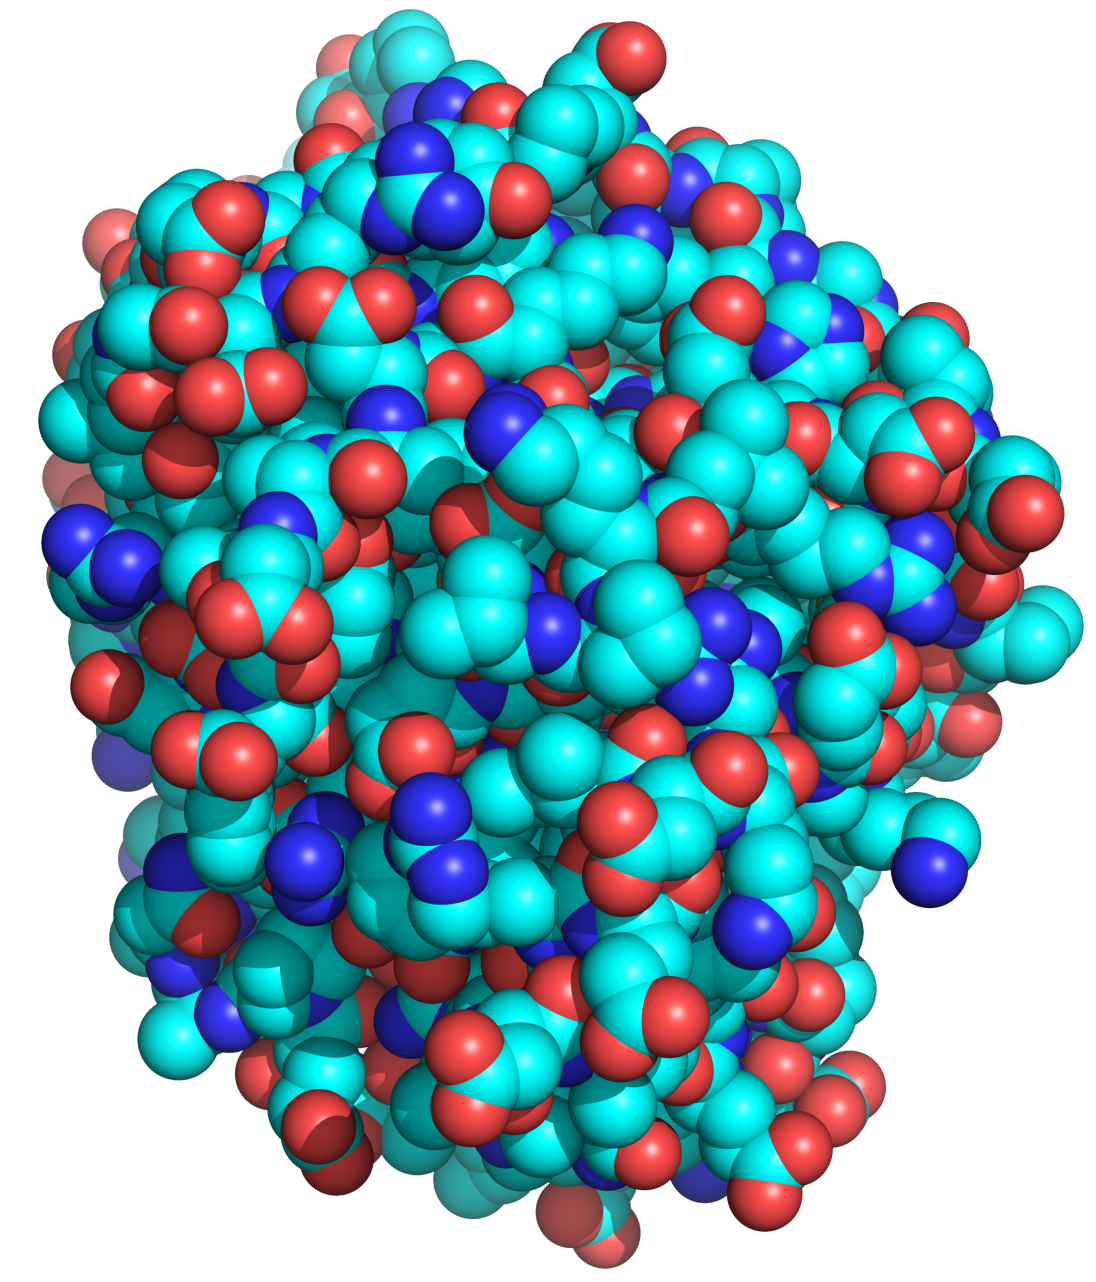
\includegraphics[width=0.15\textwidth]{fig/motiv1} &
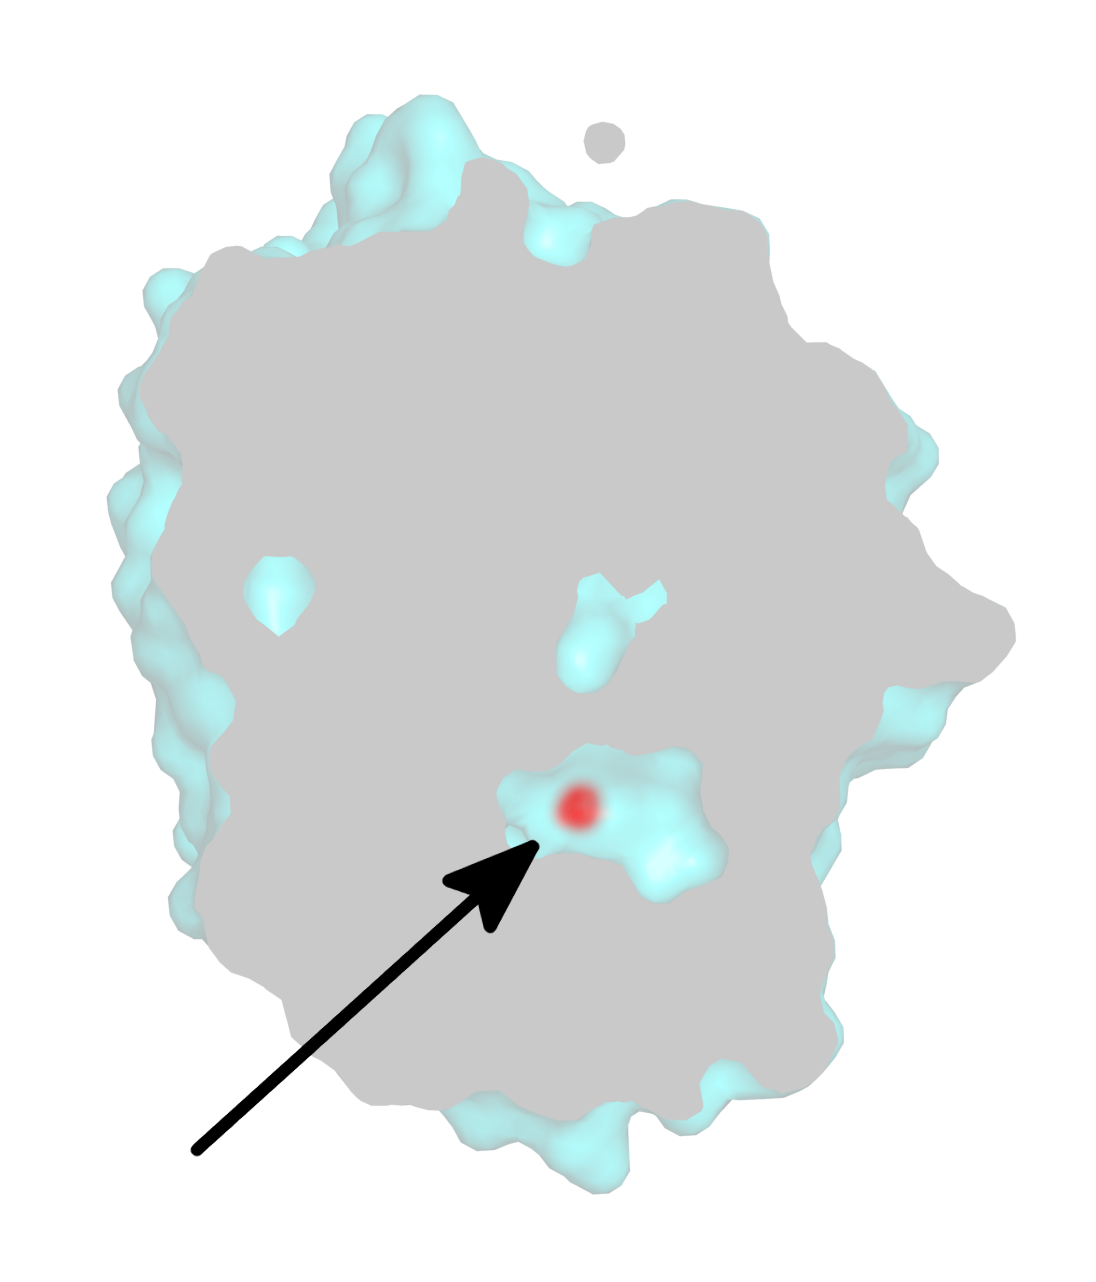
\includegraphics[width=0.17\textwidth]{fig/motiv2lab} \\
%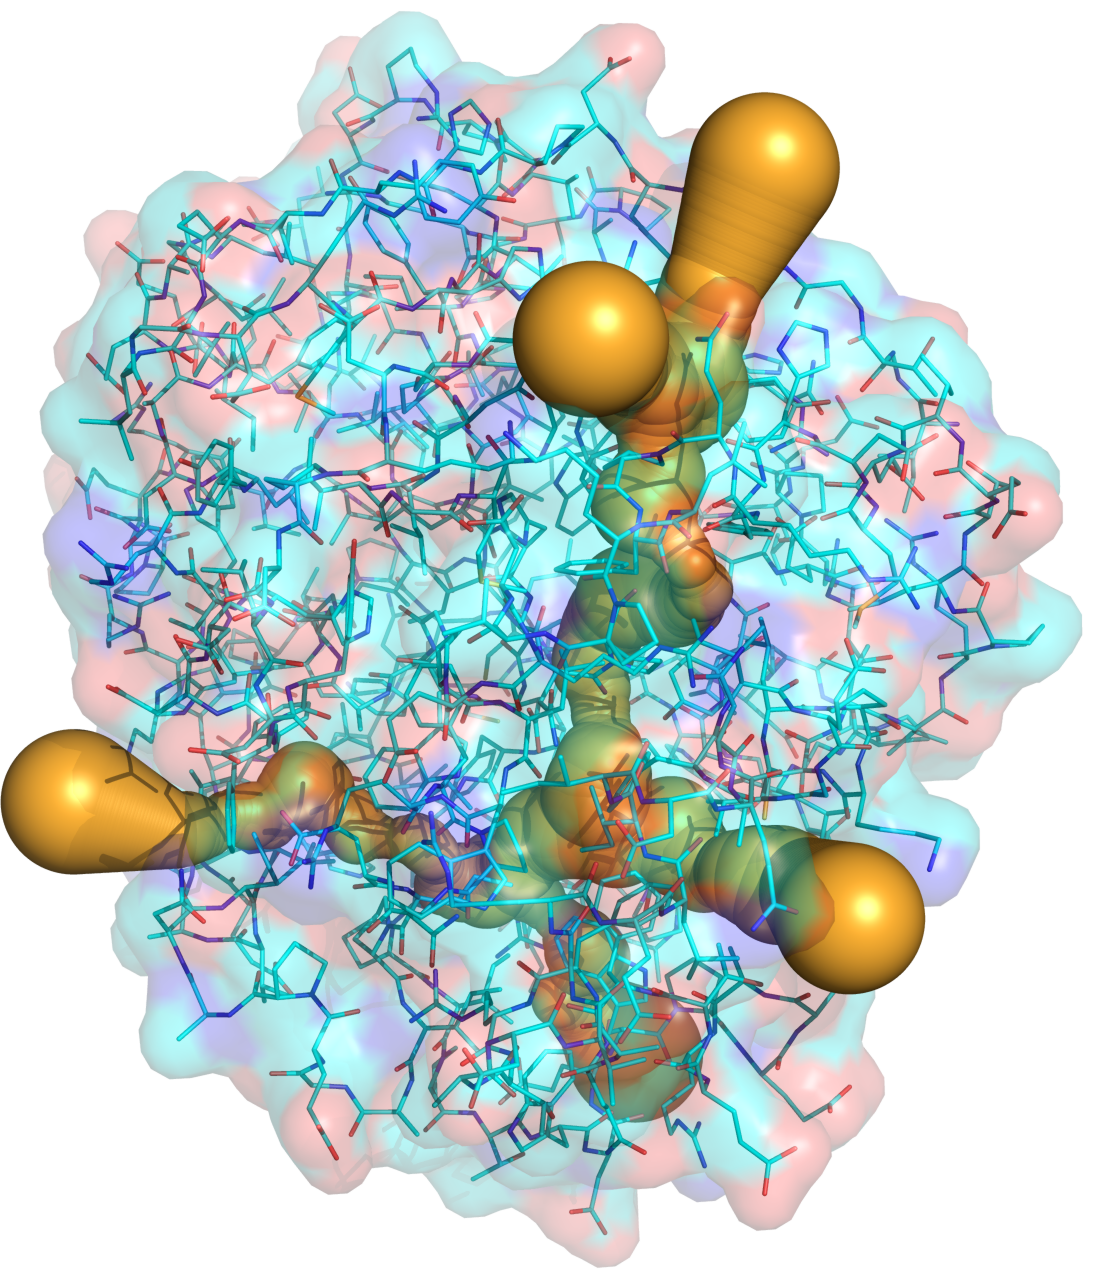
\includegraphics[width=0.16\textwidth]{fig/motiv3} \\
Protein 1CQW & Active site & Detected tunnels \\
             &            & (orange)
\end{tabular}
}
\caption{\label{fig::motiv}
    Example of tunnel detection in haloalkane dehalogenase.
}
\end{figure}

Due to low volume of protein void space, sampling-based tunnel detection may suffer from the narrow passage problem.
%Building a configuration tree of a spherical probe moving in a protein is however very challenging due to low volume of the protein void space.
To cope with narrow passages, we propose to generate the samples along a subset of Voronoi vertices of the atoms.
%a novel approach that combines VD-based techniques with sampling-based algorithms.
%Instead of generating samples randomly in the whole configuration space, they are generated around a changing subset of vertices of Weighted Voronoi Diagram.
The subset is automatically adapted so it always attracts the tree towards unexplored regions of the configuration space.
The configuration tree is expanded towards the random samples and also by the Voronoi vertices.
Construction of the configuration tree only from Voronoi vertices is not suitable, as it would result in a sparse configuration tree, that would be discontinued when switching to the next frame of protein dynamics.
To enable tunnel detection among changing (moving) atoms, it is necessary to fill the void space by a dense configuration tree, which
is achieved by the randomized sampling.

%vertices of Voronoi diagram.
%The set is maintained in such a way, so it attracts the tree towards unexplored parts of the Voronoi diagram.


%To prevent the tree growth outside the protein, which could lead to detection of invalid (outer) tunnels, we propose
%to block its growth using a set of blocking spheres.
%This results in a tree representing collision-free configurations inside the protein.
%Before the tree is used in the next frame, its nodes that collide with new positions of atoms are removed.
%It is therefore ensured, that for each node in each frame, a path leading to the starting node in the first frame can be found in the tree.
%a path between each node and the starting configuration can be found in the sequence of
%trees.
%It is therefore ensured, that all configurations in the tree are connected to the starting configuration in the first frame.

%The tunnels have low volume compared to the volume of the whole protein, which may slow down sampling-based planning.
%We propose several modifications to RRT to cope with this problem.

%Moreover, RRT allows us to easily cope with additional constraints
%As the biomolecules are densely filled with atoms, their tunnels behave like narrow passages.
%To cope with this problem, we propose two novel modifications of RRT.


\section{Related work}

The analysis of protein structure aiming to reveal the tunnels has been supported by different computational software tools which take the geometry of the protein as an input and explore the inner void space (e.g., CAVER 1.0~\cite{citeulike:6257975} or MOLE~\cite{Petrek20071357}). 
Early methods for tunnel detection utilized a discretized 3D grid, where each cell is considered as occupied or free depending
on the presence of atoms of the protein.
Tunnels can be then searched using standard graph-search methods like Dijkstra's algorithm.
Besides, the grid can be used to identify other relevant properties like 
pockets, cavities, or channels~\cite{sehnal2013mole,citeulike:6257975}.
%One of the first grid-based approaches to the detection of tunnels in protein is the CAVER 1.0 algorithm by Pet\v{r}ek et al.~\cite{citeulike:6257975}.
The obvious disadvantage of the grid-based methods is the high memory demand and their dependency on the grid resolution.
Due to the high memory consumption, these methods are not suitable for tunnel detection in dynamic proteins and therefore they
are used primarily for analysis of static molecules or individual snapshots of dynamics.

%hese approaches are not suitable for tunnel detection in dynamic proteins, a
%, which limits the usage of these methods for spherical ligands.
%To increase precision by 10, the number of cells increases by $10^3$.
%Another disadvantage is that the 3D grid does not consider orientation of the ligand and therefore, the computations 
%are useful only for spherical ligands.

Currently the most widely used approach to tunnel detection is based on Voronoi diagrams (VD) or Weighted Voronoi Diagrams (WVD).
The ordinary VD is computed on points representing centers of all atoms, without considering radii of the atoms.
This may lead to detection of tunnels with incorrect bottlenecks. % i.e., incorrect radius of a smallest probe that can traverse the tunnels.
To consider atoms with different radii, weights of individual points are determined by the van der Walls radii of the atoms in WVD.
An alternative solution is to compute a non-weighted VD on an extended point set, where 
each atom is approximated by several spheres with small radius~\cite{yaffe2008,caver3}.
%In this case, each atom is approximated by several spheres with small radius~\cite{yaffe2008,caver3}.
%The VD-based methods remove one of the main limitations of the grid-based approach which is the dependency on the grid resolution.
VD-based methods are memory less demanding, and also faster than grid-based methods.
%They can be easily used for static tunnel detection, as they are based on Voronoi diagrams of static frames.
%The grid-based and VD-based methods are usually employed on static proteins.
%Finding tunnels through time-changing proteins increases the dimension of the space to be searched, which prevents the grid-based methods
%to be used for this task.
The extension of VD-based methods to dynamic molecules requires to construct VD in the frames being analyzed and 
finding correspondences between them.
The existing approaches often use hierarchical clustering to match Voronoi vertices and edges from different frames, which is computationally demanding~\cite{lindow2012dynamic,caverDetails}.
%The main limitation of this approach is that this solution builds a complex and large hierarchical tree which has to be stored in memory and subsequently traversed which is computationally demanding. %~\cite{lindow2012dynamic}.


The tunnel detection in dynamic proteins can also be formulated as path planning in 4D (i.e., 3D $\times$ time) 
configuration space assuming a spherical probe.
%Tunnel detection in dynamic proteins leads to path planning 
%in a high-dimensional configuration space (4D for the probe and 7D for the ligand).
This space can be searched using sampling-based motion planning methods.
%Instead of a systematic search, which would be time and memory consuming, randomized sampling can be used
%to obtain necessary information about the configuration space. %~\cite{Lav06}. 
%Path planning approaches studied in robotics can be used to solve tunnel detection~\cite{guieysse2008structure} as well.
%Sampling-based path planning methods like Probabilistic Roadmaps (PRM)~\cite{kavrakiPRM} and Rapidly Exploring Random Trees (RRT)~\cite{lavalleRRT} are able to find feasible paths for complex objects with arbitrary geometries.
The idea of sampling-based motion planning is to randomly sample the configuration space $\C$ of the robot. % (i.e., the spherical probe in this case).
%The configuration space is a space of all possible configurations of the robot.
The random samples are classified as free or non-free using collision detection and  the free ones are stored into a roadmap.
A path in the roadmap then represents a motion in the workspace.
%The usage of collision detection for classification of samples allows the application of sampling-based methods for path planning for robots (objects) of arbitrary shapes.
%As the sampling-based methods work in the configuration space, they can cope with objects (robots) of many degrees of freedom
% and arbitrary shapes.
%Sampling-based planners have been used in various applications in robotics~\cite{elbanhawi2014sampling} and also  %,latombe1999motion} and also
% to study proteins, e.g. in  
%loop motions~\cite{cortes2004geometric},
%protein folding~\cite{amato2002using,raveh2009rapid,novinskaya2015improving,songPFintro},
%protein folding~\cite{raveh2009rapid,novinskaya2015improving},
%or protein folding combined with ligand diffusion~\cite{cortes2010simulating}.
Rapidly Exploring Random Tree (RRT)~\cite{lavalleRRT} is a single-query motion planning method.
RRT incrementally builds a configuration tree $\T$ rooted at the initial configuration.
In each iteration of RRT, a random configuration $\qrand \in \C$ is generated and its nearest node in the tree $\qnear \in \T$ is found.
A new configuration $\qnew$ is constructed on the line connecting $\qnear$ and $\qrand$ in the distance $\varepsilon$.
If $\qnew$ is collision-free, it is added to the tree.
The algorithm terminates if the tree approaches the goal configuration close enough.

Beyond robotics, sampling-based motion planners have been successfully applied in computational biology in studies
related to 
protein folding~\cite{al2012motion,gipson2012computational,cortes2010simulating,amato2002using,raveh2009rapid,novinskaya2015improving,songPFintro}, or analysis of loop motions~\cite{cortes2004geometric}.
%rrt for molecular: \cite{al2012motion}
%survey \cite{gipson2012computational}
Solutions for tunnel detection using sampling-based methods however have not been discussed yet.
The most relevant paper is~\cite{guieysse2008structure}, where RRT is used to compute pathways for flexible ligands towards 
the active site.
This method however does not compute explicitly all tunnels, rather a single pathway.

In our recent paper~\cite{vonasek2016application}, we have proposed to detect tunnels using RRT.
In this approach, RRT samples the configuration space of a small spherical probe moving in a single frame of protein dynamics.
After the tunnels are found in one frame, the built  configuration tree is transferred to the next frame of protein dynamics and pruned to remove
nodes colliding with the new positions of atoms.
This results in a sequence of connected trees, that can be searched for path representing the tunnels in the protein dynamics.

%This allows us to build a sequence of trees, where each tree corresponds to each frame of protein dynamics.
%The nodes of the trees are connected to their parents in the same frame, or to their parents in the previous frame.
%This allows us to find paths in this sequence of tree between two given frames, that correspond to the dynamic tunnels.

In comparison to~\cite{guieysse2008structure}, the approach~\cite{vonasek2016application} assumes spherical probes, which is motivated
by practical reasons.
%The tunnels can be computed for a spherical probe or even for non-spherical ligands --- small molecules.
%Computing tunnels considering only spherical probes is more practical.
%Despite the ability of sampling-based planners to find path for robots (objects) of arbitrary shapes, which is achieved by the collision detection, the above described approach~\cite{vonasek2016application} detect tunnels only for spherical ligands.
%The reasons are practical.
Flexible ligands have many degrees of freedom, which increases dimension of the configuration space to be searched and makes
the collision-detection more complex.
Moreover, it is required to define suitable metric and possibly also an efficient data structure for nearest-neighbor search.
%Dimension of the configuration space of flexible ligands is higher and it is determined by the Degrees Of Freedom of the ligand.
%It is required to define proper metric to efficiently search this space using RRT.
%Planning patways for flexible ligands leads to a search in a high-di
%Taking into account flexible ligands increases the dimension of the configuration space.
Despite the flexibility of ligands, their movements in proteins are strongly limited, as they are typically larger than spherical
probes.
Traversability of the ligand through a protein may depend on its initial orientation, 
 which can further limit the growth of the configuration tree.
Contrary, configuration space of  spherical probes is only 3D with the possibility to employ Euclidean metric and KD-trees for the
nearest neighbor search.
It is more practical to first detect tunnels for a spherical probe and then analyze traversability of the actual shape of ligand.
In this case, the traversability analysis is limited only to a tunnel and its vicinity, which decreases volume of the configuration space and
decreases the number of atoms involved in collision detection.
%which is faster than searching path for the ligand in the full protein.

%The ability of RRT to quickly explore the configuration space is caused by the combination
%of uniform sampling and the nearest-neighbor rule used to select nodes for the expansion.
The growth of the configuration tree into some regions of the configuration space can however be slowed down due to the narrow passages.
A narrow passage is a small region of the configuration space containing part of the solution.
As the samples are generated from uniform distribution in RRT, probability of placing the samples into the narrow passages is low and therefore,
   the probability of expanding the tree through a narrow passage is small~\cite{hannaWIS}.
%Due to its low volume, the probability of expanding the nodes towards the passage is small~\cite{hannaWIS}.
%    many iterations are needed before a tree can be built through the passage~\cite{hannaWIS}.
A possible solution is to estimate the location of narrow passages from the knowledge of the workspace and generate more samples
in the difficult areas.
For Probabilistic Roadmaps~\cite{kavrakiPRM}, this can be achieved simply by generating more samples in the difficult areas, e.g. along
medial axis~\cite{wilmarthMAPRM,foskey01hybrid,guibas1999probabilistic,hoff2000interactive,yang2004adapting}.
%This requires to precompute the medial axis, which can be time consuming.
%Another approach is to shift the random samples towards the medial axis~\cite{amatoOBPRM} or into a direction of estimated
%medial axis~\cite{hollemanMAPRM}.
Generating random samples in difficult regions however does not ensure construction of a better tree in the case of RRT-based methods. 
In RRT, the configuration tree is expanded in the direction of random samples, but the obstacles may prevent to reach them closely~\cite{vonasekphd}.
Increased probability of sampling in a given region, e.g., in a narrow passage, 
brings advantage only if the tree is close to the region and if it can reach it.

In this paper, we propose how to combine RRT-based search with Voronoi-based methods in the task of tunnel detection. 
To guide the configuration tree using Voronoi diagram, a subset of Voronoi vertices is determined and
the samples are generated around vertices in this subset.
The subset is maintained according the distance from the tree, so the random samples
are generated only if they are in a suitable distance from the tree.
This allows us to sample simultaneously along all promissing parts of VD that are accessible from the tree, which is 
suitable for detection of multiple tunnels.


%In this paper, we propose how to combine the VD-based methods and sampling-based approaches for tunnel detection.
%Instead of uninformed sampling of the configuration space, which has been proposed in~\cite{vonasek2016application}, we propose
%to generate the random samples using Voronoi diagrams.


%~\cite{amatoOBPRM,hollemanMAPRM} shift random samples towards medial axis of the environment, which helps to sample
%narrow passages more densely. 
%For example, the random samples generated in the configuration space can be shifted
%towards the medial axis of the environment~\cite{amatoOBPRM,hollemanMAPRM} or even generated around the medial 
%axis~\cite{wilmarthMAPRM,foskey01hybrid,guibas1999probabilistic,hoff2000interactive,yang2004adapting}.
%The paper~\cite{amatoOBPRM} suggests to sample uniformly in the configuration space and shift the samples towards the medial axis.
%Another approach is to generate the samples randomly in \CS\ and shift them closer to the medial axis~\cite{amatoOBPRM}.
%The medial axis can be computed exactly using GVD.
%While the medial axis can be easily computed for 2D or 3D workspaces using GVD, its computation become complicated in many dimensions.
%In such case, the samples can be generated uniformly from the whole \CS\ and moved in an estimated direction towards the medial axis~\cite{hollemanMAPRM}.



%sampling-based for 
%protein-ligand access and docking \cite{bayazit2001ligand,singhLig,apaydin2004stochastic,cortes2010simulating}
%protein and RNA folding~\cite{amatoPF1,ApaBru03}
%protein loop motions~\cite{cortes2004geometric},
%domain motions~\cite{kirillova2008an}, 
%and motions of pairs of alpha-helices in transmembrane proteins~\cite{enosh2007prediction}

%The tree is extended from a node, that is selected as a nearest node to a randomly generated configuration in the configuration space.
%The highest probability of expansion have nodes with large Voronoi cells. 
%Due to this Voronoi-bias, the tree grows towards unexplored regions of the configuration space.
%However, the Voronoi-bias brings disadvantages in narrow passages.
%nodes in the narrow passages.



%The behavior of RRT in the narrow passages was analyzed using Voronoi diagrams in~\cite{yershovaDDRRT}.
%The nodes in the tree can be divided into two groups: frontier nodes, whose Voronoi cells grow together with growth
%of the environment and boundary nodes, which are close to the obstacles. %~\cite{yershovaDDRRT}.
%The tree cannot be expanded from the boundary nodes.
%In a narrow passage, the nodes are both boundary and frontier.
%These nodes are frequently selected for the expansion, because they are the frontier nodes, however the tree cannot be expanded
%from them, because they are also the boundary nodes. 
%To suppress selection of the boundary nodes, authors of~\cite{yershovaDDRRT} suggest to define an action radius around each node.
%The node is selected for the expansion only if its radius is larger than the distance to the random sample.
%The radius of new nodes is set to $\infty$ and it is decreased to a predefined value $\rdd$ if the node cannot be expanded.
%A Dynamic-Domain strategy for RRT (RRT--DD) is proposed in~\cite{yershovaDDRRT}:
%each node holds an action radius defining how far can be a random sample $\qrand$ that activates the node for the expansion.
%The RRT--DD algorithm generates random samples $\qrand$  and finds its nearest neighbor in the tree
%$\qnear$ until $\rho(\qrand,\qnear) < \qnear.radius$. 
%Although the algorithm is efficient in the narrow passages, it is strongly influenced by the parameter $\rdd$.
%To decrease the sensitivity of the method to the parameter $\rdd$, it can be automatically adjusted, which
%was proposed in RRT--ADD (RRT with Adaptive Dynamic Domain)~\cite{jailletATDDRRT}.
%Another schema to automatically adjust parameters of the RRT-based planners was proposed in~\cite{schneider2015completely}.

%Retraction-RRT~\cite{zhangRetraction} generates random samples uniformly as in the original RRT, but it
%attempts to shift them into the narrow passages.
%A~random configuration $\qrand \in \CF$ is generated and a close non-free configuration $q \in \CO$ is found. 
%A~contact configuration $q_c$ on a segment $(\qrand,q)$ is found and its neighborhood is searched for
%$q_c'$ minimizing the distance between $q$ and $q_c'$. 
%The configuration $q_c'$ is then added to the tree.
%It was shown that this approach can deal with narrow passages efficiently,
%because the generated contact configurations penetrate into the narrow passages.
%However, to find the contact configurations, the collision detection algorithm is called frequently, which can decrease
%the performance of the algorithm.

%The goal-bias principle can be further extended by sampling the configuration space along a path computed in the workspace~\cite{vonasek2009rrt,amatoOBRRT}.
%%Geometric path in the workspace~\cite{vonasek2009rrt} or medial axis of the 3D space~\cite{amatoOBRRT} can be used to guide the tree.
%Sampling along geometric paths constructed in the workspace is suitable for low-dimensional configuration spaces, e.g. for
%path planning of mobile robots.
%However, the geometric paths computed in workspace are less effective for sampling in high-dimensional configuration spaces~\cite{hannaWIS}.
%



%of the narrow passages is related to narrow passaged of the workspace~\cite{hannaWIS}.
%
%is to manipulate the random samples, e.g. to change their rotation, rotation or both parts or to shift them closer to the medial
%axis of the workspace~\cite{amatoOBPRM}.

%In~\cite{amatoOBPRM} several strategies for validating non-free random samples have been proposed.
%Authors propose different manipulation procedures for random configurations generated during the learning phase.
%For example, the random configuration can be placed into the roadmap with changed rotation, translation or both, or it can be
%shifted away from an obstacle allong a line connecting the sample and medial axis of the obstacles.
%In a configuration is invalid, it is pushed randomly into various directions to gen free samples around boundaries of $\CO$.





% ===============================================================================


%25\% of VDW radii, T-RRT \cite{jaillet10costmap}

%\red{The tunnel detection task differs from classic motion planning it two main aspects: a) the goal configuration
%is not explicitly defined, and b) multiple pathways (tunnels) should be detected.}


%Molecular structures can be represented as articulated bodies and sampling-based methods can be used
%Path planning methods have been used to expore the conformational space of 
%proteins~\cite{novinskaya2015improving,songPFintro,mollProt,proteinRRT},
%Other applications of sampling-based approaches is in detection of 
%folding pathways~\cite{amato2002using}, analyzing protein loops~\cite{cortes2004geometric}, 
%or modeling large-scale transitions in a protein structure~\cite{raveh2009rapid}
%The geometric-based tunnel detection approaches provide fast computation of tunels in large protein structures and they
%have been integrated in several tools like Caver~\cite{bara2014caver}, Chexvis~\cite{masood2015chexvis} and other.
%Most of the proposed methods consider only spherical models of ligand~\cite{benkaidali2014computing}.

%dxTuber: Detecting protein cavities, tunnels and clefts based on protein and solvent dynamics:
%furtng protein cavities, tunnels and clefts based on protein and
%solvent dynamics insights into the protein in question. For example, empty
%space in a protein structure can provide valuable insight into protein properties such as internal hydration, structure stabilization,
%substrate translocation, storage compartments or substrate binding sites [1,2]. This information can be visualized by means of cav-
%ity analysis. Over the years numerous cavity detection tools have been developed including [3–17] that depict cavities either directly
%[3–6,8,10–17] or indirectly by identifying lining residues [9] or filling a cavity with water molecules [7]. The main strategies used
%in these geometry-based algorithms [1] can be grouped into four categories plus combinations of these.
%n the motion planning problem, that is widely studied in robotics, the task is to find a feasible trajectory for a robot between two

%given positions in an enironment.
%To utilize the motion planning approaches, the ligand is considere as the robot and the protein's atoms as the obstacles.
%Computing feasible (traversable) tunnels for non-spheric ligands requires to consider also rotations of the ligands, which 
%can be solved using sampling-based approaches like Probabilistic Roadmaps (PRM)~\cite{kavrakiPRM} or Rapidly Exploring
%Random Trees (RRT)~\cite{lavalleRRT}.
%Sampling-based methods randomly samples configuration space of the robot (ligand) and the samples are classified
%as free or non-free using collision detection.
%The free samples are stored in a graph structure.
%A path in the grap then corresponds to a motion in the workspace.



%In~\cite{guieysse2008structure}, RRT method is used to compute pathways for flexible ligands.


%\cite{lindow2012dynamic}
%Analysis of protein dynamics suggests that internal cavities and channels can be rather dynamic structures. 
%Voronoi-based algorithm to extract the geometry and the dynamics of cavities and channels from a molecular dynamics trajectory.
%The algorithm requires a pre-processing step in which the Voronoi diagram of the van der Waals spheres is used to calculate the cav-
%ity structure for each coordinate set of the trajectory. 
%In the next step, we interactively compute dynamic channels by analyzing the time evolution of components of the cavity structure. Tracing of the
%cavity dynamics is supported by timeline visualization tools that allow the user to select specific components of the cavity structures
%for detailed exploration. All visualization methods are interactive and enable the user to animate the time-dependent molecular struc-
%ture together with its cavity structure. To facilitate a comprehensive overview of the dynamics of a channel, we have also developed a
%visualization technique that renders a dynamic channel in a single image and color-codes time on its extension surface. 
%
%
%Sampling-based motion planning algorithms from the field of robotics have been very successful in exploring the
%conformational space of proteins
%\cite{novinskaya2015improving}
%Sampling-based algorithms explore the conformational space of a protein by randomly sampling it (usually using a special
%heuristic) and constructing a graph where each node represents a feasible low-energy protein conformation (or state), and each
%edge represents a possible low-energy local transition between two states. 
%The computed graph describes the topology of a protein’s energy landscape and the connectivity of its lowenergy areas. 
%This graph can be used to find possible large-scale transitions between two given protein conformations.
%

%Sampling-based methods have been very effective for the fast computation of representative motions of molecular systems \cite{al2012motion, gipson2012computational}


%A broad range of approaches exploit sampling-based techniques to address various biological problems, such
%as exploring energy landscapes \cite{devaur2014sampling} ,
%modeling protein folding pathways \cite{amato2002using}, analyzing protein loops \cite{cortes2004geometric}, 
%or modeling large-scale transitions in a protein structure \cite{raveh2009rapid}

%In computational biology, molecules and proteins are modeled as articulated bodies and sampling based planners are used to simulate
%protein folding and protein-ligand interactions  \cite{al2012motion} 
%asi spis necitovat \cite{gipson2012computational}



%Ms have been applied to model molecular motions by modeling the molecule as an articulated linkage and 
%replacing the typical collision detection validity check with some measure of physical viability (e.g., potential energy).
%Protein motions, ranging from molecular flexibility to large-scale conformational change, play an essential role in many biochemical processes. 
%!!to map transitinos between specific conmfotrmations!!!!
%ample conformation space more effectively, and we describe extensions of our framework to automate
%the process and to map transitions between specified conformations.
%\cite{thomas2006simulating}
%

%In subsequent work, our group used another PRM variant on this problem \cite{bayazit2001ligand}
%Our group was the first to adapt PRMs to model protein folding pathways 
%\cite{amato2003using, amato2002using, song2003apath}

%Using a standard modeling assumption for proteins that bond angles and bond lengths are fixed \cite{sternberg1996protein}, 
%the only dof in our model are the backbone’s phi and psi torsional angles which are modeled as revolute joints with values 0 .. 2pi

%
%The roadmap produced by our technique is an approximation of the protein’s energy landscape. 
%Roadmap quality is measured both by how realistic (as compared to experimental data) its pathways are and by how many samples are required
%to achieve the desired accuracy. 
%The latter is important because it determines what size molecules can be analyzed.
%Hence, sampling is the key to producing a good approximation of the land-scape. 
%Note that only a relatively small portion of the conformation space ‘near’ the target conformation(s) is of interest in modeling motions. 
%This implies that we should use biased sampling to cover the regions of interest efficiently.
%
%genrovani lepsich vzorku: using rigidity analysis~\cite{thomas2006simulating}
%or perturbing:
%iterative sampling process where we apply small Gaussian perturbations to existing conformations~\cite{amato2003using, amato2002using, song2003apath}
%
%rrt for tunnel (pathway) detection
%\cite{cortes2010simulating}
%\cite{corset2005path}
%\cite{guieysse2008structure}
%

%Many modifications have been proposed for RRT to speed up the growth of the tree~\cite{kuffnerRRTC}, 
%     to consider an optimality criteria such as path length~\cite{karaman2011sampling}, and to improve behavior in narrow passages~\cite{amatoOBRRT,vonasek2009rrt,zhangRetraction,schneider2015completely}. 
%For example, RRT--Retraction~\cite{zhangRetraction} analyzes the line segment from $\qnear$ to $\qrand$.
%If the line segment is collision-free, the tree is expanded normally using the straight-line planner.
%Otherwise, the contact configuration on the line segment is constructed and its neighborhood is searched
%for other contact configurations in order to minimize the distance to $\qrand$.
%This retraction step allows RRT--Retraction to place the nodes of the tree into narrow passages.



%The behavior of RRT in the narrow passages was analyzed using Voronoi diagrams in~\cite{yershovaDDRRT}.
%The nodes in the tree can be divided into two groups: frontier nodes, whose Voronoi cells grow together with growth
%of the environment and boundary nodes, which are close to the obstacles. %~\cite{yershovaDDRRT}.
%The tree cannot be expanded from the boundary nodes.
%In a narrow passage, the nodes are both boundary and frontier.
%These nodes are frequently selected for the expansion, because they are the frontier nodes, however the tree cannot be expanded
%from them, because they are also the boundary nodes. 
%To suppress selection of the boundary nodes, authors of~\cite{yershovaDDRRT} suggest to define an action radius around each node.
%The node is selected for the expansion only if its radius is larger than the distance to the random sample.
%The radius of new nodes is set to $\infty$ and it is decreased to a predefined value $\rdd$ if the node cannot be expanded.
%A Dynamic-Domain strategy for RRT (RRT--DD) is proposed in~\cite{yershovaDDRRT}:
%each node holds an action radius defining how far can be a random sample $\qrand$ that activates the node for the expansion.
%The RRT--DD algorithm generates random samples $\qrand$  and finds its nearest neighbor in the tree
%$\qnear$ until $\rho(\qrand,\qnear) < \qnear.radius$. 
%Although the algorithm is efficient in the narrow passages, it is strongly influenced by the parameter $\rdd$.
%To decrease the sensitivity of the method to the parameter $\rdd$, it can be automatically adjusted, which
%was proposed in RRT--ADD (RRT with Adaptive Dynamic Domain)~\cite{jailletATDDRRT}.
%Another schema to automatically adjust parameters of the RRT-based planners was proposed in~\cite{schneider2015completely}.

%Retraction-RRT~\cite{zhangRetraction} generates random samples uniformly as in the original RRT, but it
%attempts to shift them into the narrow passages.
%A~random configuration $\qrand \in \CF$ is generated and a close non-free configuration $q \in \CO$ is found. 
%A~contact configuration $q_c$ on a segment $(\qrand,q)$ is found and its neighborhood is searched for
%$q_c'$ minimizing the distance between $q$ and $q_c'$. 
%The configuration $q_c'$ is then added to the tree.
%It was shown that this approach can deal with narrow passages efficiently,
%because the generated contact configurations penetrate into the narrow passages.
%However, to find the contact configurations, the collision detection algorithm is called frequently, which can decrease
%the performance of the algorithm.


%Another approach to biased sampling was presented in~\cite{bruceERRT}, where the trajectories found in previous
%iterations are used to sample the configuration space. 
%This modification is suitable for dynamic environments.

%The growth of the tree can be attracted into a region $\R \in \C$ by increasing probability of sampling in that region.
%This is used in the goal-bias principle~\cite{lavalleRRTPP}, where $\qgoal$ is used instead of $\qrand$ with the probability $\gb$.
%The goal-bias suppresses the exploration of $\C$ and the tree is expanded more preferably towards the goal.
%An extension of the goal-bias was presented in~\cite{kardossRRTKK}, where a predefined key-configuration is 
%used to focus sampling to difficult areas of the configuration space.
%%Authors suggest to place the key-configuration in a way that connects easy and difficult areas of the configuration space.
%%For example, the key-configuration can be placed at the enter to a narrow passage.
%%Although the goal-bias speeds up the growth towards the goal, it may cause a congestion problem of the tree growth due to existence of an obstacle in the pathway.
%
%
%The goal-bias principle can be further extended by sampling the configuration space along a path computed in the workspace~\cite{vonasek2009rrt,amatoOBRRT}.
%%Geometric path in the workspace~\cite{vonasek2009rrt} or medial axis of the 3D space~\cite{amatoOBRRT} can be used to guide the tree.
%Sampling along geometric paths constructed in the workspace is suitable for low-dimensional configuration spaces, e.g. for
%path planning of mobile robots.
%However, the geometric paths computed in workspace are less effective for sampling in high-dimensional configuration spaces~\cite{hannaWIS}.
%


\section{Preliminaries}

Proteins are represented by the hard sphere model, where the radius of each sphere (atom) is given by its van der Waals radius.
Let $\SS \subset \mathbf{R}^3$ denote the union of all spheres, i.e., the geometry of the protein.
%We further assume that a subset of atoms located at the surface, are known. These atoms, reffered to as {\sl surface atoms} in this paper,
%   can be detected as atoms located at $\alpha$-shape of the molecule.
The tunnels need to be found for a spherical probe $\Sprobe$ of radius $\probe$.
%We further consider a spherical probe $\Sprobe$  of radius $\probe$ encapsulating the ligand.
Let $q=(x,y,z)\in\C$ denote the configuration (position) of the probe, where
the configuration space $\C$ consists of all possible configurations.
For each configuration $q\in\C$ we assume, that its largest collision-free radius $r(q) \in \mathbf{R}, r(q)\ge 0$ can be computed, e.g.
using collision detection.
%using collision detection.
%Let $L(q) \subseteq \mathbf{R}^3$ denote the geometry of the ligand at position $q \in \C$.
%Similarly to geometry of molecule, the geometry of ligand is union of hard sphere model.
%A probe is represented by one sphere of radius $\probe$.
The collision-free region $\CF \subseteq \C$ is formed by configurations, where $\Sprobe$ can be placed without any collision, i.e., 
$\CF = \{q \in \C | \Sprobe(q) \cap \SS = \emptyset\}$, where $\Sprobe(q)$ is the sphere with radius $\probe$ at configuration $q$.
%We assume, that atoms located on the surface of the molecule are known, these are reffered to as {\sl surface atoms}.
The distance $\dist(q_1,q_2)$  between two configurations $q_1,q_2\in\C$ is measured using 3D Euclidean metric.

%This radius can be detected using collision detection method.
The configurations outside the protein $\CG \subseteq \C$ are collision-free with sphere $\Sgprobe$ of radius $\gprobe$, $\gprobe> \probe$,
$\CG=\{q\in \C| \Sgprobe(q) \cap \SS = \emptyset \}$.
%A configuration $q \in \CG$ is referred to as {\sl goal configuration} in the rest of the paper.
By computing $\alpha$-shape of the molecule, we can identify atoms located at the surface. 
These atoms are referred to as {\sl surface atoms} in the rest of the paper.
The distance between a configuration $q \in \C$ and its nearest surface atom is referred to as $\dists(q)$.
%We assume, that for each configuration $q$, the largest collision-free radius $r(q)$ can be computed.
%Let $r(q)$ denote the radius of the largest collision-free sphere at configuration $q$.

Dynamic proteins are represented by a sequence of $n$ snapshots (frames).
The tunnels change with the protein dynamics as well: their width and position change, they can merge with other tunnels
or even disappear.
The free region $\CF$ is therefore different in each frame, as positions of atoms change.
For the sake of simplicity, a single notation $\C$ resp. $\CF$ is used in this paper and it is valid for the frame being processed.

Approximated WVD diagram of the atoms is computed by representing each atom using 12 balls of equal radii and computing ordinary Voronoi diagram.
Computing WVD this way is more efficient and numerically stable and it is used also in other related tools~\cite{caver3,yaffe2008}.
Vertices of this WVD are filtered out if their distance to an atom is less than probe radius $\probe$.
Let $\VV$ contain the remaining Voronoi vertices, and let $r_v \in \VV$ denote the distance to the nearest atom.
%The remaining Voronoi vertices $\VV$ of the WVD and their distances $r_v, v\in \VV$ to the nearest atom are then used in the following method.


%\section{Tunnel detection}

%The tunnel detection using motion planning leads to search in 4-dimensional $\C\!\times\!time$ space, which can be searched using randomized sampling-based methods.
%The task of tunnel detection is to find a collision-free path from a given starting point located inside a dynamic protein 
%to the outer environment. %: for a probe $\Sprobe$.
%The idea of the proposed approach is to detect tunnels in each frame separately using a novel modification of RRT algorithm.
%The configuration tree built in a given frame is transferred to the next frame, where the search continues.

%We propose to detect the tunnels in this 4D space
%(the space consists of pairs $(q,t) \in \C \times [1,n]$, where $n$ is the number of frames) by randomized sampling.
%where $\C$ is three-dimensional configuration space
%of the spherical probe and $n$ is the number of frames.
%It is not computationally feasible to discretize the space to a grid, in which a path is found using standard space-search methods.
%Moreover, finding a collision-free path in the space does not solve the problem, because the probe cannot move back in time.
%Tunnel detection in dynamic proteins leads to search in $\C \times time$ space. %~\cite{Kindel00kinodynamic}.
%sometimes called state-time space~\cite{berg2005roadmap}.
%The proposed solution samples the configuration space of each frame separately in order to detect possible tunnels in the frame.
%The resulting tree is then pruned to remove collision with atoms of the next frame.


\section{Tunnel detection}

The tunnel detection problem is defined by specifying the coordinates of the active site $\qinit \in \CF$, 
    the radius $\probe$ of the probe, and the radius 
$\gprobe$ that determines outer space $\CG$ of the protein.
The dynamic proteins are searched for tunnels in a two-stage process: first, the tunnels are searched in a single frame, then the
built configuration tree is transferred to the next frame and pruned.
Due to space limit, this paper focuses mainly on the first stage. 
We refer to~\cite{vonasek2016application} for detailed description of the second stage.

\subsection{Sampling of configuration space of a single frame}

%The configuration space is sampled using the RRT method. 
%The tunnels detection requires to find tunnels only inside the protein, not on its surface.
%However, proteins have jagged surface with protrusions and small cavities. 
%The growth of the tree outside the protein needs to be prohibited.
%Otherwise, many invalid tunnels hidden in this bumpy surface would be detected.
%These cavities are smaller than $\Sgprobe$ but larger than $\Sprobe$, which prevents us to determine
%configurations at the surface using simple collision detection between $\Sgprobe$ and the protein surface.
%Therefore, simple collision detection between $\Sgprobe$ and the protein may fail to determine configurations located at the surface
%of the protein.

The configuration space is searched using the RRT principle~\cite{lavalleRRT}, which is extended by three main modifications.
First, the tree expanded by several new nodes in each iteration, in order to boost growth in the narrow passages.
The second modification is designed to block growth of the tree outside the protein, which is necessary to prevent detection of false
tunnels. 
The last modification is the novel VD-based sampling of configuration space.
The proposed method is listed in Alg.~\ref{alg::tunnel}.

Instead of adding only a single node in each iteration, which is done in original RRT, we expand the tree by $m$ nodes.
This improves the growth of the tree inside the narrow passages, as these are filled by the tree in less number of iterations.
After a node $\qnear$ for the expansion is determined, its neighborhood in the distance $\varepsilon$ is sampled.
The collision-free samples (i.e., $r(q) \ge \probe$)  are stored in the set $N$.
%These configurations are randomly sampled around $\qnear$ in the distance $\varepsilon$ and these are stored in the set $N$.
%After $\qnear$ is found in the tree, its neighborhood is sampled by at most $m$ random samples in the distance $\varepsilon$. 
%These samples are stored in the set $N$ and added to the tree if they are not too close to the protein surface.
%Otherwise, blocking spheres are added at the corresponding configuration.
%a sample $q$ with the maximal collision-free radius $r(q)$. % (Fig.~\ref{fig::expansion}b,c).
The configuration $q \in N$ is added to the tree if it does not regress to the tree.
% $r(q) \ge \probe$ and 
A sample $q$ is regressing if its nearest neighbor in the tree is closer than $\qnear$. %parent node. % (Alg.~\ref{alg::lexp}, line 7).
This regression test prevents the expansion to large sites, that are already filled with other nodes. 
Without this test, the tree would densely occupy large areas, but less densely the small ones.
Tree expansion by multiple nodes result in more dense trees. 
%If $\qnew$ is located in a large area, i.e., $r(\qnew) > \probe$, additional $m$ samples located around $\qnew$ are added to
%the tree. % (Alg~\ref{alg::lexp}, lines 15--22), which is depicted in Fig.~\ref{fig::expansion}d.
%This procedure expands the tree by multiple nodes (at most $m+1$), but it guarantees that these nodes
%are collision-free at radius at least $\probe$ and that these are not regressing towards the tree.

%The active sites are typically connected with the protein's surface using multiple tunnels.
%It is therefore desired to detect as many tunnels as possible.
%On the other hand, not all path within the protein are considered as good tunnels, e.g. the tunnels partly located in the protrusions and 
%small cavities of the protein surface.
%Such tunnels, despite they are connected with the active site, are not relevant for chemists.


The active sites are typically connected with the protein’s surface by multiple tunnels.
It is therefore desired to detect as many tunnels as possible. 
On the other hand, not all paths within the protein are biochemically relevant, e.g., long thin tunnels with highly curved trajectory or
tunnels partly located on the surface of the protein.
Such tunnels, despite they are connected with the active site, are not relevant because there is a 
high probability that they will be closed in molecular dynamics.

To prevent the growth of the tree on the bumpy surface and to boost searching of tunnels inside the protein,
 algorithm searches the configuration space in two phases.
 In the first phase, { blocking spheres} $\SB$ of radius $\gprobe$ are placed
to configurations that are believed to be close to the surface.
The distance of each configuration $q \in N$ from the nearest surface atom is determined and $q$ is
added to the tree only if this distance is larger than $\ths$. 
Otherwise, $q$ is added to $\SB$ (Alg.~\ref{alg::tunnel}, line 21), because a tunnel can exit around $q$ from the protein.

%Each node $q \in N$ is therefore tested for being close to surface atoms before it is added to the tree (Alg.~\ref{alg::tunnel}, line 20).
%If this distance is less than the threshold $\ths$, the configuration $q$ is considered as being close to the surface, which
%indicates that a tunnel can exit from the protein around this point.
%Therefore, new blocking sphere at this position is introduced into the set $\SB$. % (Fig.~\ref{fig::timexp}d).

After a predefined fraction of iterations (parameter $\alpha$ in Alg.~\ref{alg::tunnel}, lines 32--35), the algorithm
switches to the second phase, and the blocking atoms $\SB$ are deleted and removed from collision detection data structures.
In this second phase, the configuration tree is allowed to exit the protein and reach the outer space.
%This allows the tree to finally expand out of  the protein.
%In such a case (lines 24--26 in Alg.~\ref{alg::tunnel}), $q$ is added to the set of tunnel exit-points.
An exit from the tunnel is detected if $q \in N$ is collision-free with sphere $\Sgprobe$ (or $r(q) > \gprobe$). 
The exit points are stored in the set $G$ (Alg.~\ref{alg::tunnel}, line 28--30).
%The algorithm can be initialized with a non-empty set $\SB$ (line 1 in Alg.~\ref{alg::tunnel}), which allows to block the growth of the tree according to exit-points detected in the previous frame.

%The second modification aims to improve the expansion step.
%Tunnel are narrow passages and the straight-line expansion of the tree, that is often used in RRT-based planners,
%to collision (Fig.~\ref{fig::expansion}a).
%In RRT literature, the tree is often expanded using the straight-line expansion, i.e., $\qnew$ is constructed on a line
%connecting $\qnear$ and $\qrand$ in the distance $\varepsilon$ from $\qnear$.
%The protein void space is small and this type of expansion would lead to collisions. % (Fig.~\ref{fig::expansion}a).
%To cope with this issue, it is necessary to find $\qnew$ around $\qnear$ and not only on the line 
%from $\qnear$ to $\qrand$. % (Alg.~\ref{alg::lexp}).

\linesnumbered
\begin{algorithm}[h]
%\setstretch{\straa}
{\small
\caption{\label{alg::tunnel}static tunnel detection}
\KwIn{Initial configuration tree $\T$,
    initial set of blocking spheres $\SB'$
}
\KwData{goal-probe radius $\gprobe$,
    probe radius $\probe$, 
    max. number of iterations $\Imax$, 
    phase switching threshold $\alpha$,
    threshold $\ths$,
    num. of new nodes $m$ in each iteration,
    prob. $\gb$ of sampling randomly from $\C$
}
\KwOut{Configuration tree $\T$,
    list of tunnel exit-points $G$
}
\hrule
$\SB = \SB'$; //blocking atoms added during phase~1 \\
$G = \emptyset$; // list of tunnel exit-points \\
$phase=1$\;
\For{$iteration = 1:\Imax$}{
    \If(// Voronoi-based sample --- Section~\ref{sec::vbg}){$phase=1$}{
        $\VVA =$ update active Voronoi points from $\VV$\;
        $v =$ random point from $\VVA$\;
        $\qrand =$ random point around $v$ in the distance $r_v$\;
%        $a_1$ = random atom on surface\;
%        $a_2$ = random atom on surface\;
%        $\qrand$ = random point on line $|a_1, a_2|$\;
    }
    \If{$rand() < \gb$}{
        $\qrand$ = random sample from $\C$\;
        $v = \emptyset$; //no Voronoi vertex used
    }

    $\qnear$ = nearest node in $\T$ towards $\qrand$\;

    \If{$v \ne \emptyset$ {\bf and} $\dist(\qnear, v) < \probe$} {
        add $v$ to $\T$, set its parent to $\qnear$\;
    }

    $N\!=\!m$ collision-free nodes around $\!\qnear$ in the distance $\!\varepsilon$\;
%    $(\qnew,r(\qnew))$ = expand($\T$,$\qnear$, $\SS \cup \SB$)\;
    \For{$q \in N $}{
        \eIf{$\dists(q) < \ths $ {\bf and} $phase=1$}{
            $\SB = \SB \cup \{\Sgprobe(q)\}$ \;
        }{
            $q'$ = nearest node in $\T$ towards $q$\;
            \If{$\dist(q,q') > \dist(q,\qnear)$}{
                add $q$ to $\T$, set its parent to $\qnear$\;
            }
        }
        \If{ $r(q) > \gprobe$ }{
            $G = G \cup \{ q \} $\;
        }
    }
    \If{$phase = 1$ {\bf and} $iteration > \alpha \Imax$}{
        $phase = 2$\;
        $\SB = \emptyset$; // block. atoms are not used in phase 2 \\
    }
}
\return $(\T, G)$\; 
}
\end{algorithm}

%\begin{algorithm}[h]
%%\setstretch{\straa}
%{\small
%\caption{\label{alg::lexp}expand()}
%\KwIn{Configuration tree $\T$, configuration $\qnear$ to be expanded, 
%    collision-geometry $\SS$
%}
%\KwData{num. of random samples $n$ around $\qnear$, 
%    max. number of additional nodes $m$,
%    resolution $\varepsilon$
%}
%\KwOut{Return new node $\qnew$ and its collision-free radius $r(\qnew)$ if it is added to tree, or NULL otherwise
%}
%\hrule
%    $\qnew = \emptyset$; // new node to be added to the tree \\
%    $r' = 0$; // largest collision-free radius of node $\qnew$\\
%    \For{$i=1:n$}{
%        $q$ = random sample around $\qnear$ in distance $\varepsilon$\;
%        $q'$ = nearest node in $\T$ towards $q$\;
%        $r(q)$ = collision-free radius of sample $q$ w.r.t. $\SS$\;
%        \If{$dist(q,q') < dist(q,\qnear$) {\bf and} $r(q) > r'$}{
%               $r' = r(q)$\; 
%               $\qnew = q$\;
%        }
%    }
%    \If{$\qnew \ne \emptyset$}{
%        $\T$.addNode($\qnew$)\;
%        $\T$.addEdge($\qnear, \qnew)$\;
%        \If{$r' > \probe$}{
%            $r_{s} = r' - \probe$\;
%            \For{$i=1:m$}{
%                $q$ = random sample in distance $r_s$ from $\qnew$\;
%                $\T.$addNode($q$)\;
%                $\T.$addEdge($\qnew, q$)\;
%            } 
%        }
%        \return $(\qnew,r')$\;
%    }
%    \return NULL;
%}
%\end{algorithm}
%

\subsection{Tunnel detection in dynamic proteins}

A sequence of frames of protein dynamics is searched by repeated construction of a tree and its transfer to the next frame.
The collisions between the nodes of the actual tree and atoms of the next frame are checked and the colliding nodes are removed.
The parents of the remaining nodes are changed to corresponding nodes from the previous tree.
The search then continues by expanding the existing tree using Alg.~\ref{alg::tunnel}.
This results in a sequence of trees.
Each node in the tree points to its parent, which is either a node of the same tree, or a node of the tree in the previous frame.
Also, the result is a set of exit points (the set $G$ in Alg.~\ref{alg::tunnel}), which contains ending points of tunnels in each frame. 
The tunnels are then reconstructed by searching paths from each $g \in G$ to the first frame (or to other frame of interest).

%The algorithm starts with the first frame at configuration $\qinit \in \CF$.
%We assume that this position is collision-free at frame $1$, otherwise it would not be possible to construct the tree around it.
%The result of the static tunnel detection (Alg.~\ref{alg::tunnel}) is a new configuration tree of collision-free nodes for frame $i$ and
%tunnel exit-points $G$.
%Further expansions from the tunnel exit-nodes have to be prohibited, otherwise the tree would fill the outer region of the molecule.
%Similarly to the Alg.~\ref{alg::tunnel}, this is achieved using the blocking spheres $\SB$.
%The blocking spheres have radius $\gprobe$ and they are placed at tunnel exit-points $G$ (Fig.~\ref{fig::timexp}d).
%The result of the Alg.~\ref{alg::tunnel} is a configuration tree $\T$ representing the protein void space, together with
%a set of tunnel exit-points $G$. 
%The result of Alg.~\ref{alg::main} is represented by a sequence of trees $\T_0,\ldots,\T_n$, and the tunnel exit-points stored in the set $G$.
%$t$ is represented by the sequence 
%$t=\left((q_1,f_1), \ldots, (q_{k},f_{k})\right)$ of $k$ points $q_i$ and their corresponding frames $f_i$.

%\begin{algorithm}
%%\setstretch{\straa}
%{\small
%\caption{tree pruning\label{alg::copyTree}}
%\KwIn{Geometry $\SS_{i+1}$ for frame $i+1$,
%    configuration tree $\T_i$ constructed at frame $i$
%}
%\KwData{probe radius $\probe$, goal radius $\gprobe$}
%\KwOut{Configuration tree $\T_{i+1}$ valid for frame $i+1$}
%\hrule
%$\SB = \emptyset $\;
%$\T_{i+1} = $empty tree\;
%\For{$q \in \T_i$}{
%    $r(q)$ = largest collision-free radius at $q$ w.r.t. $\SS_{i+1}$\;
%    \If{$r(q) \ge \probe$ {\bf and} $r(q) < \gprobe$ }{
%        $T_{i+1}.$addNode($q$)\;
%        set parent of $\T_{i+1}$.node($q$) to $\T_i.$node($q$)\;
%    }
%    \If(// $q$ is tunnel exit-point){$r(q) \ge \gprobe$}{
%        $\SB = \SB \cup \{\Sgprobe(q)\}$\;
%    }
%}
%\return $(\T_{i+1}, \SB)$\;
%}
%\end{algorithm}
%
%


\section{Voronoi-based guided sampling}
\label{sec::vbg}

Due to limited void space of the protein, tunnel detection suffers from the narrow passage problem.
To cope with this problem, we propose to guide the sampling in the configuration space using vertices $\VV$ of WVD of the atoms.
To prevent stucking of the tree due to obstacles (i.e., atoms), it is necessary to generate random samples around $\VV$ only if the tree has
a chance to grow towards the random samples.
To achieve this, we maintain a set of {\sl active} Voronoi vertices called $\VVA$. 
A Voronoi vertex $v \in \VV$ is considered as active, if the distance to its nearest node in the tree is less than $\da$, but larger than
$\db$ (Fig.~\ref{fig::av}).
The upper value $\da$ ensures, that the active Voronoi vertices are close to the boundary of the configuration tree, whilst
the lower value $\db$ prevents to activate Voronoi vertices that have already been approached by the tree.
This sampling process therefore automatically adapts according to the progress of the configuration tree:
after the tree approaches a given $v \in \VVA$, this vertex is removed from $\VVA$ so its surrounding is not sampled anymore.
Contrary, distant vertices $v \in \VV$ are not used for sampling.


To generate a random sample $\qrand$, $v \in \VVA$ is randomly selected and $\qrand$ is generated around $v$ using Gaussian distribution with 
$\sigma = r_v$ (Alg.~\ref{alg::tunnel}, lines 5--9).
%This Guassian distribution is used because it allows to generate $\qrand$ also out of the sphere ce
%so $\qrand$ can be placed also out of the sphere of the Voronoi vertex $v$.
%which has been shown to be useful.
The Voronoi-based sampling is used only in the first phase of the method, where the tree growth outside the protein is blocked by $\SB$.  
In the second phase, it is desired to grow outside the protein and the VD structure is not needed, so
 $\qrand$ is randomly taken from the whole $\C$ with probability $\gb$ (Alg.~\ref{alg::tunnel}, line 10--13).

%It should be noted, that Voronoi vertices alone does not necessary represent the tunnels, 
%as they can be located too close to the atoms (closer than the radius of the probe). 

Besides generating $\qrand$ around $v \in \VVA$, the Voronoi vertex $v$ is added to the tree if its distance to $\qnear$ is less than
 $\probe$ (Alg.~\ref{alg::tunnel}, lines 15--17).
Such addition is valid as all vertices in $\VV$ (and consequently in $\VVA$) have collision-free radius at least $\probe$.

The set $\VVA$ does not need to be updated in each iteration, because the tree is expanded only by the distance $\varepsilon$ in each
iteration. 
The update can be realized e.g. after every $k$ nodes added to the tree.

%The configuration tree is expanded by several nodes in each iteration, but in the maximal distance $\varepsilon$, so several
%terations is needed to approach a given $v \in \VVA$. 
%Therefore, it is not necessary to update $\VVA$ in each iteration, but only after $k$ nodes is added to the tree.

%As the configuration tree is extended by several spheres in each step that are at most in distance $\varepsilon$ from the expanded node $\qnear$.
%It is therefore needed several iterations to extend the tree close enough to the nodes in $\VVA$.
%Consequently, it is not necessary to update $\VVA$ in each iteration, but rather after every $k$ nodes added to the tree (Alg.

\begin{figure}
\centering
%\includegraphics[width=0.23\textwidth]{fig/activevor}
%\includegraphics[width=0.23\textwidth]{fig/activevor2}
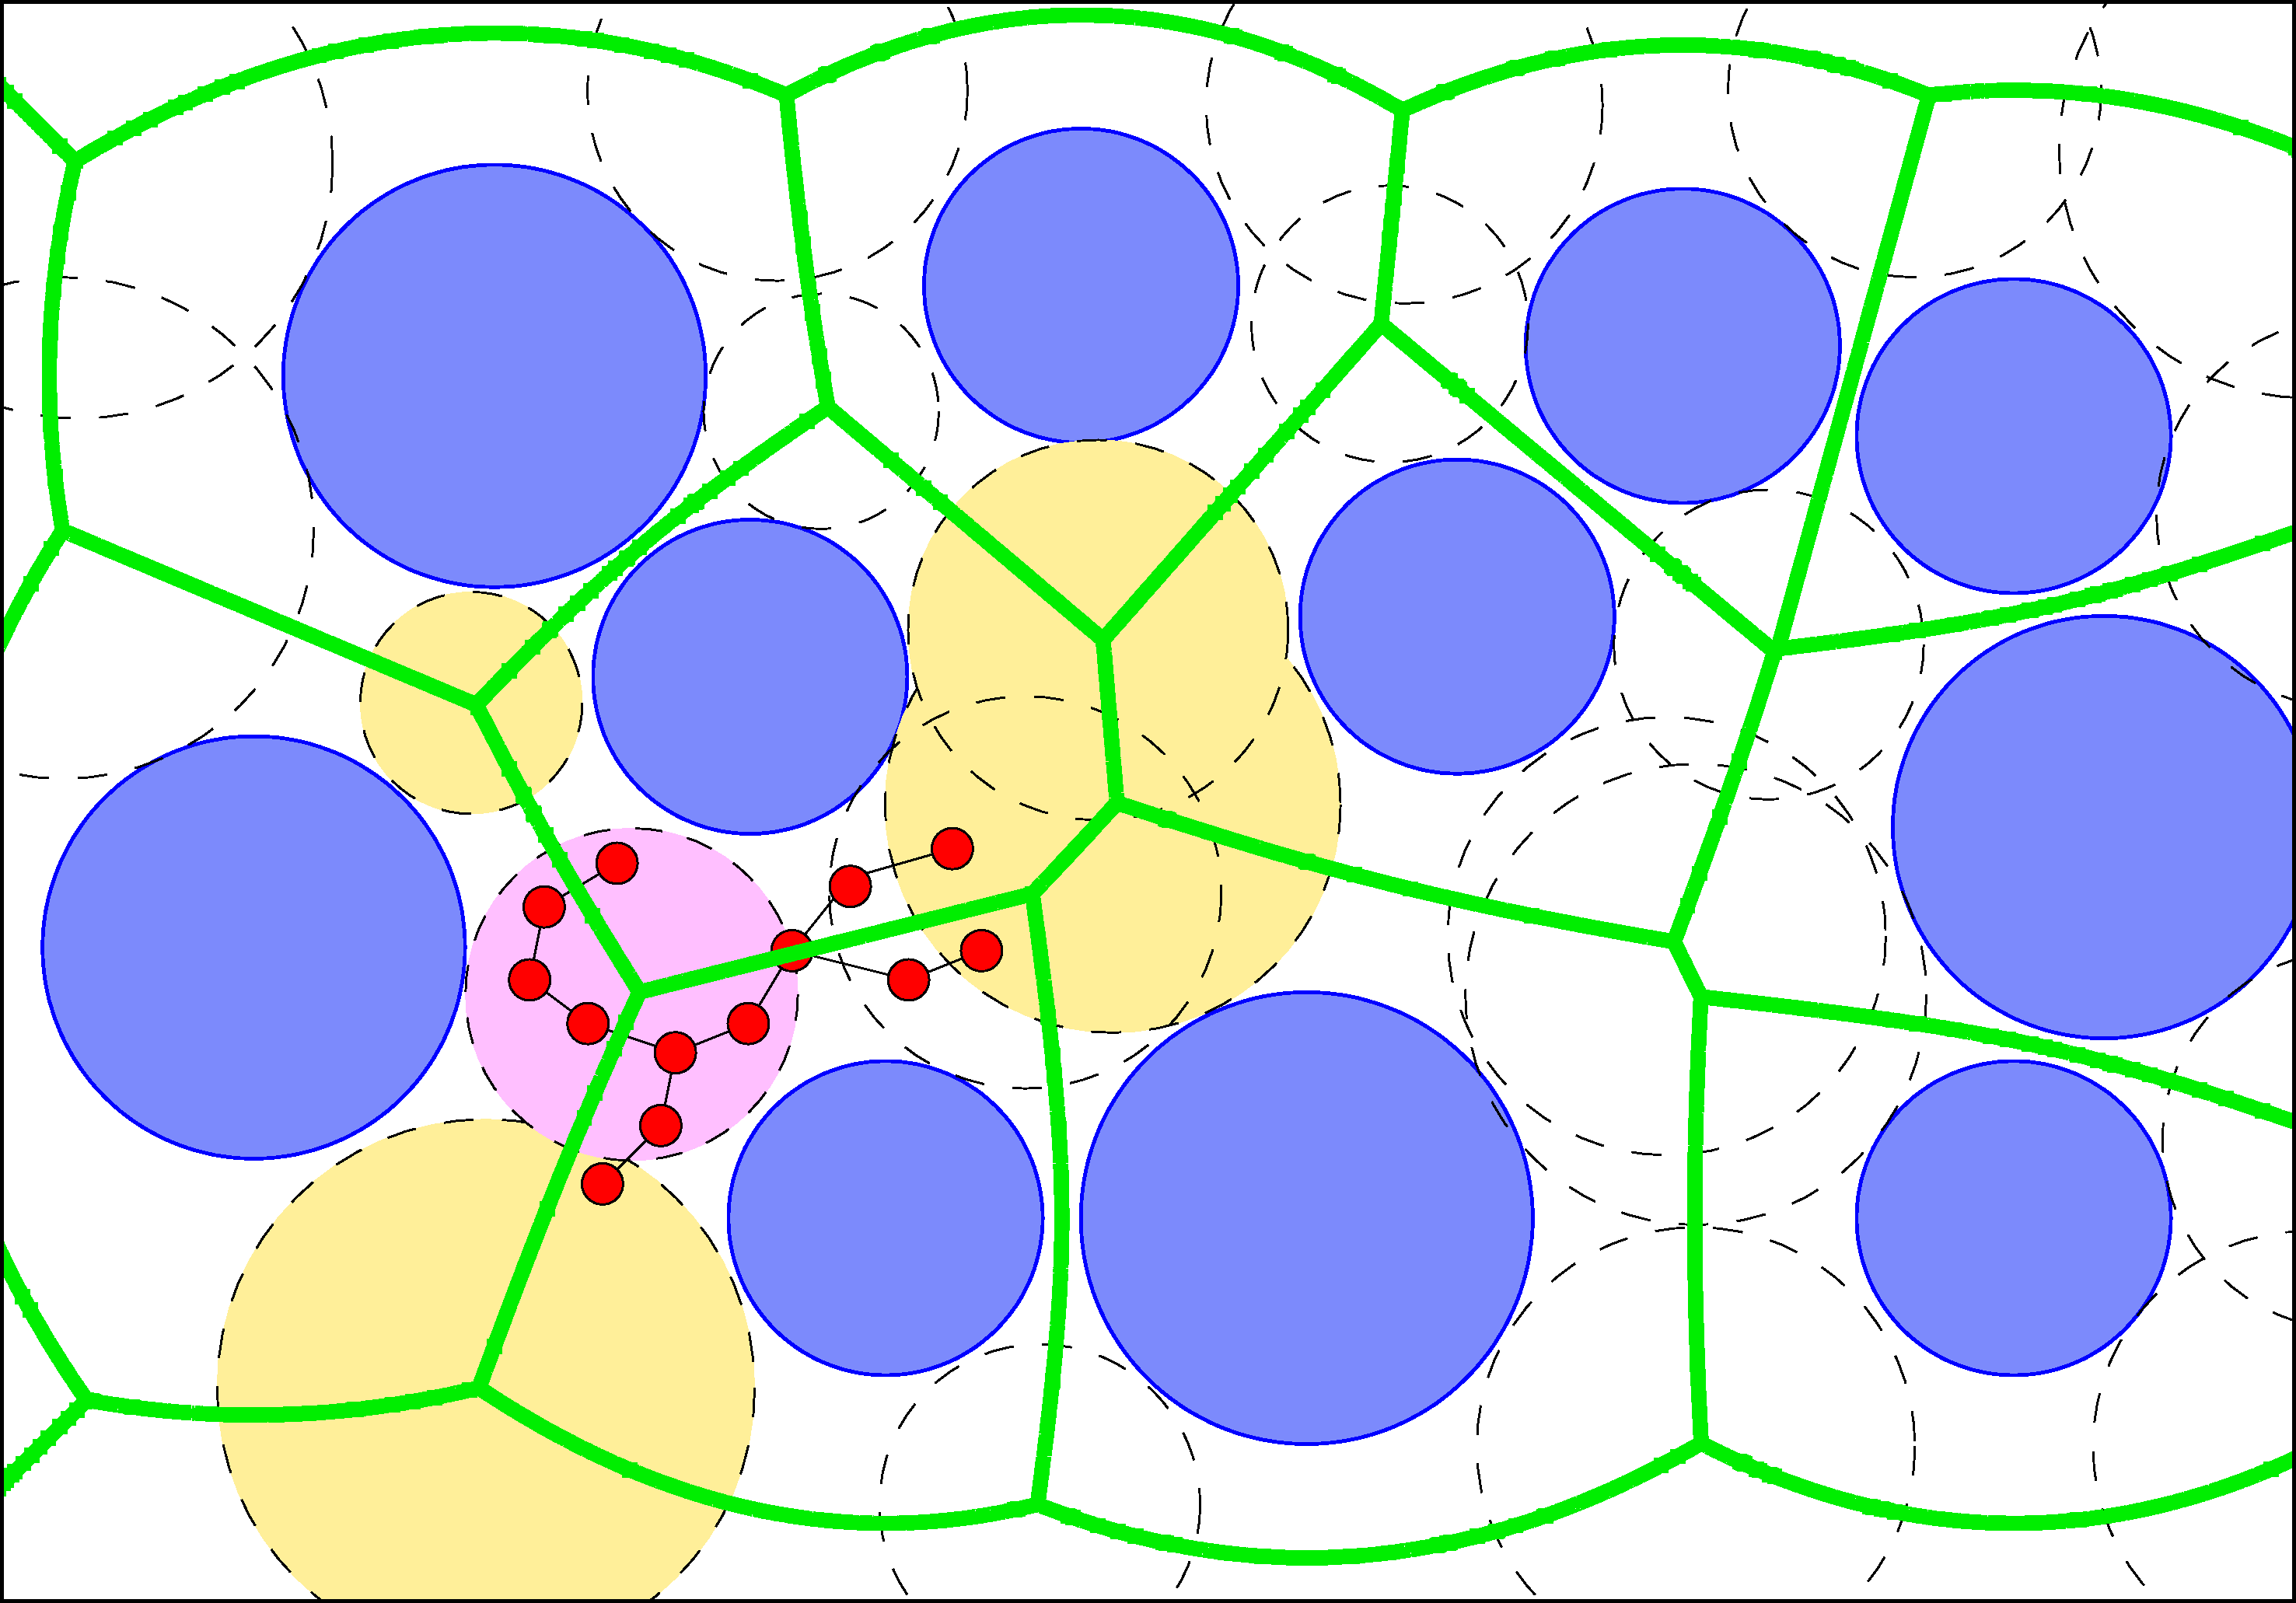
\includegraphics[width=0.23\textwidth]{fig/av1}
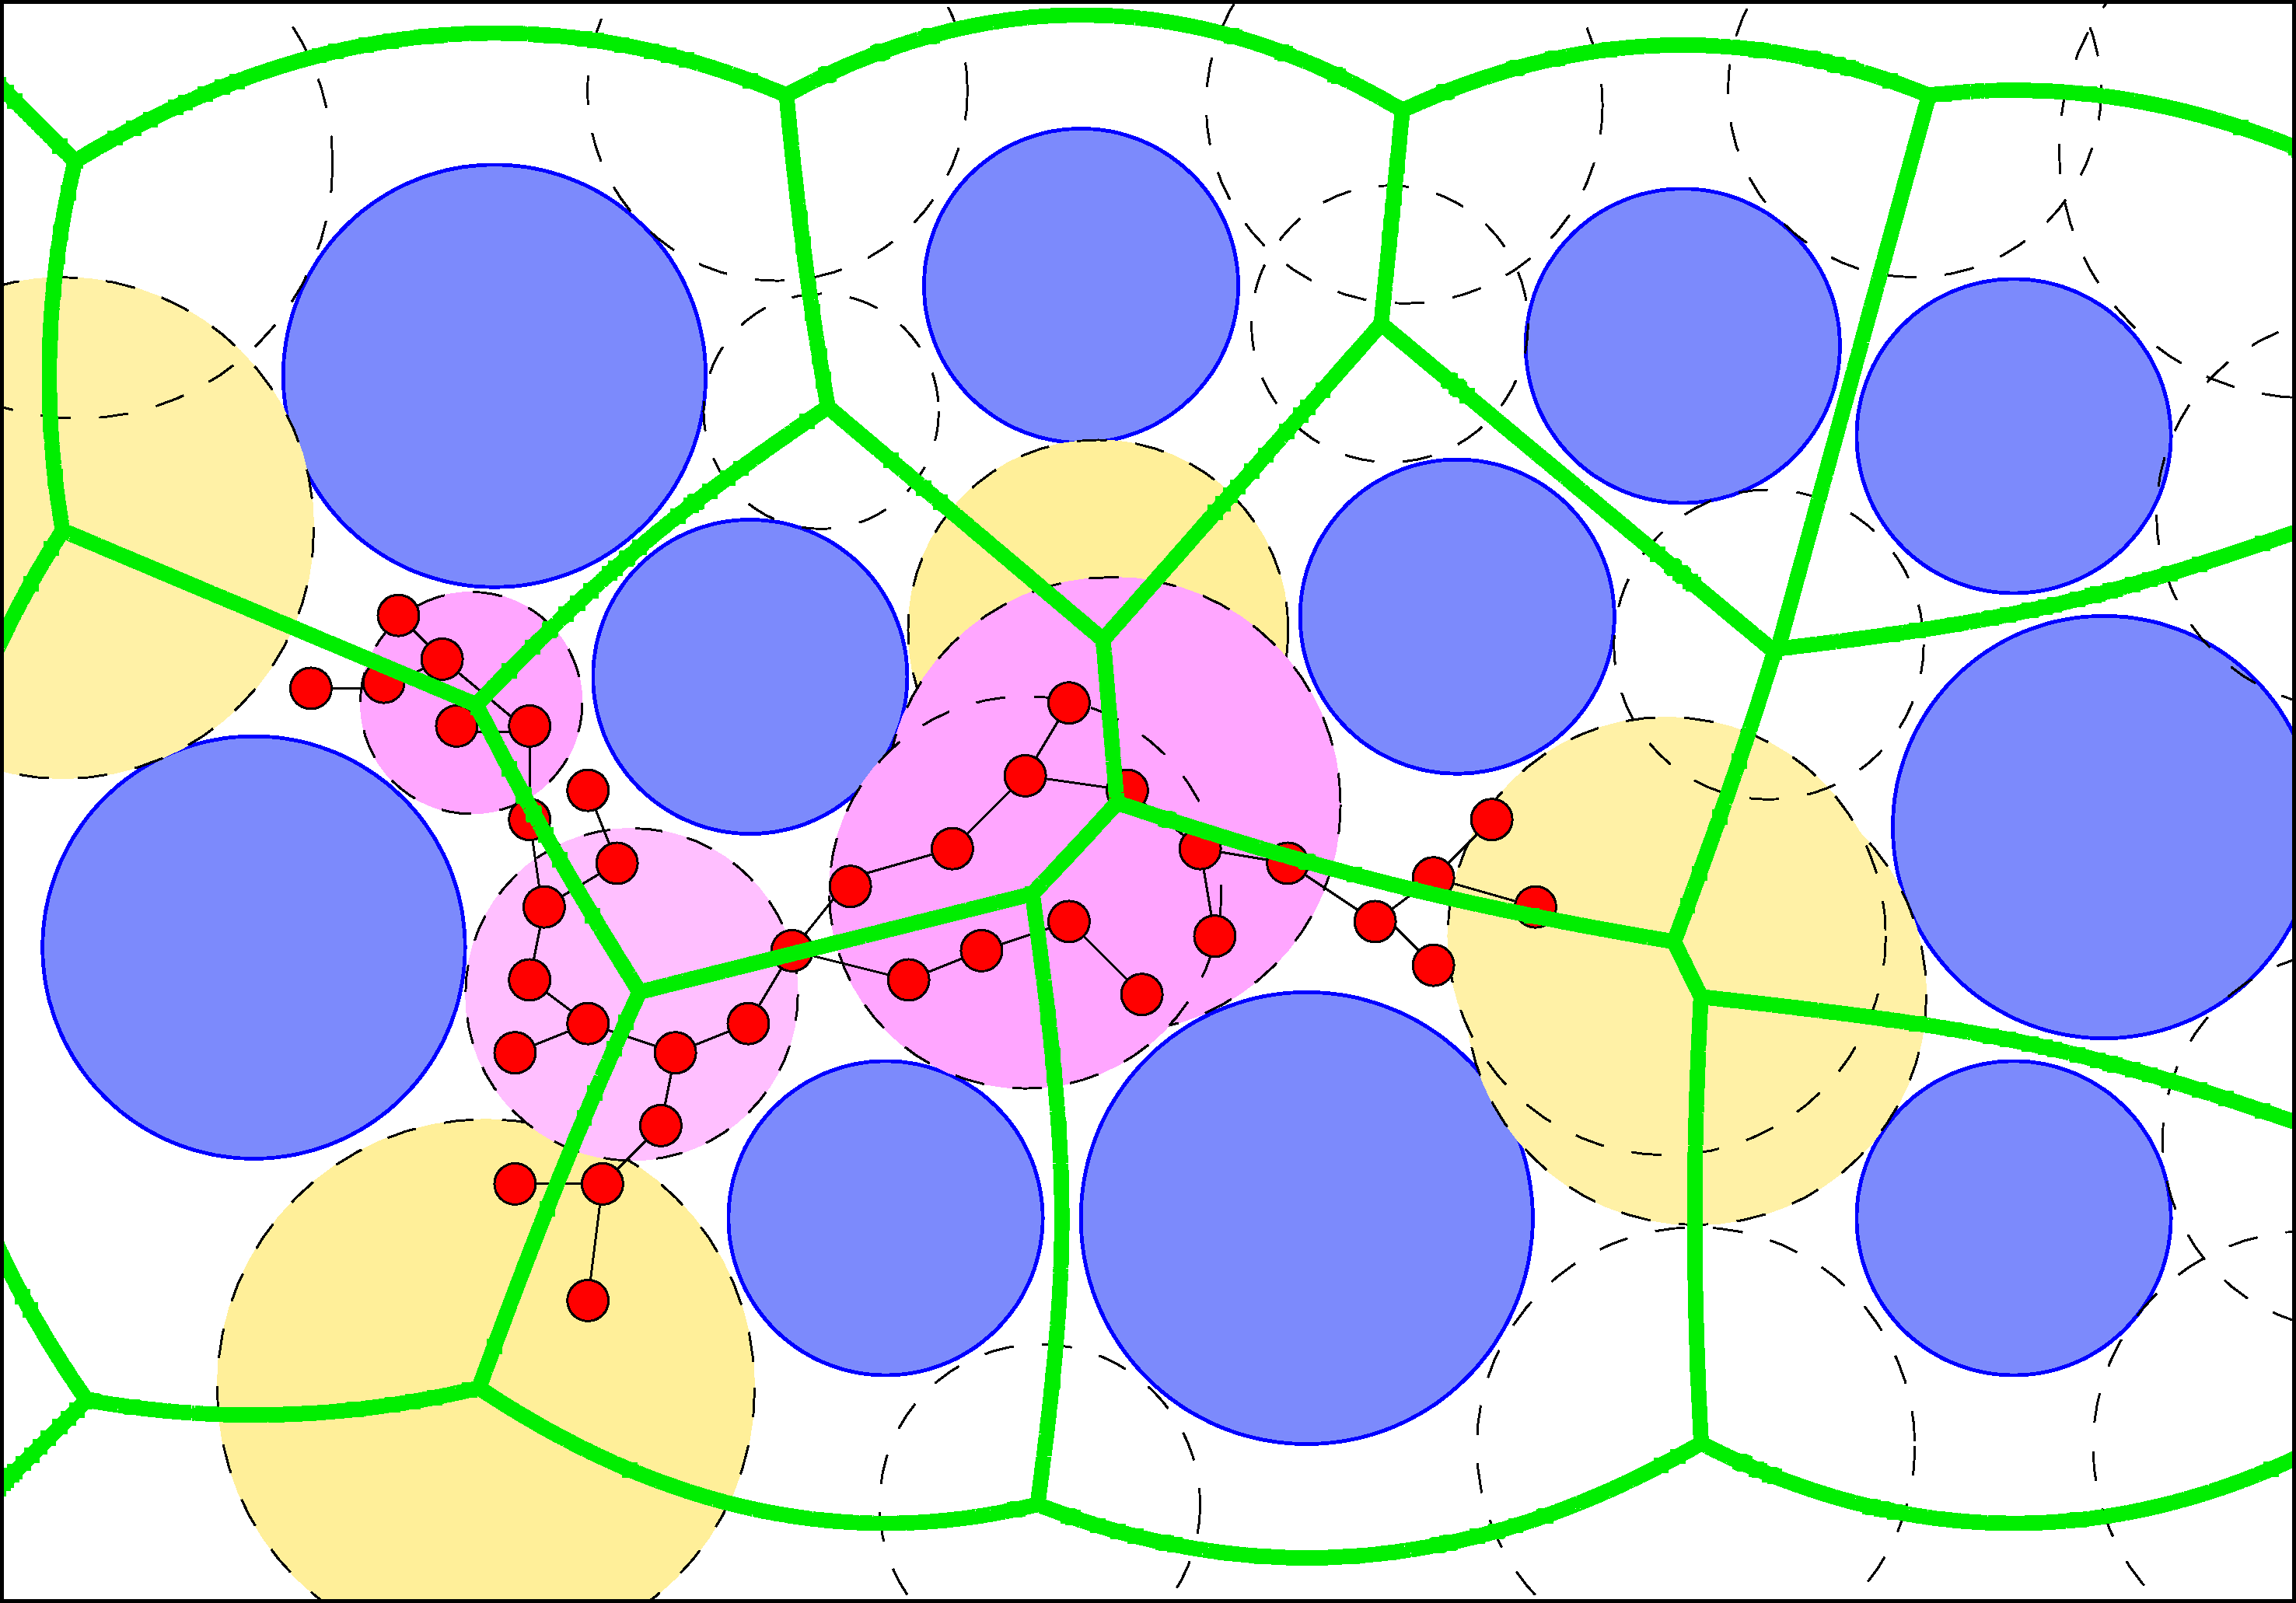
\includegraphics[width=0.23\textwidth]{fig/av2}
\caption{\label{fig::av}
    Simplified example of a progress of generating random samples using WVD of a set of 2D atoms.
    Atoms are depicted in blue, WVD edges in green.
    Dashed circles are centered at Voronoi vertices, and the radius is given by the distance to the nearest atom.
    Small red circles represent a partially built configuration tree.
    Active Voronoi vertices, that are close to the tree are depicted in light yellow.
    Random samples are generated around these active vertices.
    The tree is attracted by samples in the yellow regions (left). 
    Voronoi vertices, that have been already approached, are depicted in light pink (right).
    Random samples are not generated around these vertices, so the tree is still attracted towards unexplored regions.
}
\end{figure}

\section{Discussion}
%+proc nepridavat rovnou koule z WVD
%+multiple tunnels

%The advantage of the proposed approach is that the sequence of protein snapshots is searched frame by frame.
%By transferring the constructed tree to the next frame it is ensured that tunnels can be search not only within frame, but also
%between two given frames.

As each frame of protein dynamics is analyzed separately, only the actual configuration tree and frame-related data structures 
(e.g., WVD, collision-detection structures) need to be held in the memory.
After the frame is switched, the full tree from the previous frame can be stored.
According to our experiments, 50--70\% of nodes are kept to the next frame.
The amount of required memory therefore does not depend on the number of frames to be processed, but mainly on the size of the protein.
The sampling in the next frame does not start from scratch, but it continues by adding new nodes to the tree.
Therefore, the number of iterations $\Imax$ has to be large for the first frame in order to maximize the number of detected tunnels, but it can 
be decreased for the subsequent frames.

Detecting tunnels for spherical probes brings several advantages.
The collision detection can be computed very fast between a spherical probe and the hard sphere model of the protein.
Besides, simple 3D Euclidean metric can be used to measure the distance in the configuration space.
Consequently, the nearest neighbor search can be realized using KD-trees in $\mathcal{O}(\log n)$, where $n$ is the number of 
nodes in the tree.
KD-trees can also be used to compute the distance $\dists$ to surface atoms 
(line 20 in Alg.~\ref{alg::tunnel}), and for the update of set $\VVA$ (Alg.~\ref{alg::tunnel}, line 6), 
which makes these procedures fast.
   
%The sampling in a given frame is terminated after $\Imax$ iterations.
%The tree is then pruned to remove the nodes colliding with atoms of the next frame.
%The amount of memory required to detect tunnels in a sequence of protein dynamics is given only by the number of nodes in each frame.

The number of atoms in proteins, their arrangement as well as roughness of the surface may significantly vary, 
       and the behavior of the algorithms have to be adjusted.
The ability to detect tunnels is influenced by the parameter $\alpha$.
The first phase should be long enough in order to build the tree inside the protein.
According to experiments on proteins listed in Tab.~\ref{tab::results}, 
we suggest to set $\alpha=0.7$, i.e., 70\% of iterations is performed in the first phase.
The distance to surface atoms $\ths$ indicating tunnel exit points depends on the roughness of the protein surface and we recommend
to set it less than $\gprobe$, e.g. $\ths=\gprobe/5$ in our case.
The parameters of Voronoi-based sampling, $\da$ and $\db$ depend on the amount of void space and also on the probe radius $\probe$.
We recommend to use $\db=0.5\probe$ and $\da=4\probe$.

%For the purpose of visualization and further analysis, it is convenient to fill the spheres, i.e.,  to find $r(q_i)$ for each point $q_i \in t$.

\section{Experimental verification}

{\bf Static tunnel detection: }
The proposed method (Alg.~\ref{alg::tunnel}), referred to as \TA, is compared to~\cite{vonasek2016application} (referred to as \TB) and
to basic search of 3D path for sphere using the basic RRT~\cite{lavalleRRT}, denoted as \TC.
In \TB, the Voronoi-based sampling is not used.
%Algorithms are run with the following parameters.

%Collision detection was realized using OZCollide library~\cite{ozcollide}.
Voronoi vertices $\VV$ used in \TA\ are computed using WVD with the weight set to the radii of the atoms.
Only Voronoi vertices located inside the alpha-shape are considered to be in the set $\VV$.
The set $\VVA$ is updated after 1000 new nodes in the tree.
\TA\ and \TB\ strategies are run with $\alpha=0.7$ and $\Imax=50\cdot 10^3$ iterations.
The thresholds for Voronoi sampling in \TA\ are $\da=4r_v$ ($r_v$ is radius of a Voronoi vertex $v \in \VV$), $\db=0.5\probe$.
\TA\ and \TB\ expand the tree by up to $m=4$ new nodes in each iteration, \TC\ only by one.
\TC\ therefore needs more iterations, so for a fair comparison, \TC\ is run with 10 times more iterations ($\Imax=500\cdot10^3$).
All other settings are the same for all three tested strategies:  $\varepsilon=0.1$~\AA, $\gprobe=5$~\AA, $\ths=1$~\AA.

%(Alg.~\ref{alg::tunnel}), referred to as \RRTTD\ in the rest of the paper, 
%was launched with $\Imax=50\cdot10^3$ iterations, $\alpha=0.7$, and for probes $\probe=0.8, 0.9$, and $1.1$~\AA, resolution
%$\varepsilon=0.1$~\AA, and $\gprobe=5$~\AA, expansion parameters $n=50$, $m=3$, and $\ths=1$~\AA.
%The resulting tunnels were compared with CAVER 3.0~\cite{caver3} analytical tool that computes tunnels using approximated Voronoi diagrams.

%The proposed \RRTTD\ method was also compared with a na\"{i}ve RRT, referred to as \RRTN\ in the following text.
%\RRTN\ was implemented according~\cite{lavalleRRT} and it generates random samples uniformly in the configuration space and expands
%the tree using the straight-line expansion with resolution $\varepsilon=0.1$~\AA.
%d as RRT-na\"{i}ve in the rest of the text, gienerates random samples uniformly from the whole configuration space, and it does not use the two-phase blocking mechanisms to prevent growing of the tree outside molecules. 
%\RRTN\ builds the configuration tree slower than \RRTTD\, therefore $\Imax=500\cdot10^3$ iterations were used in \RRTN\ in order to build
%trees with similar number of nodes~as~\RRTTD.



Tunnels are searched for several proteins from the Protein Data Bank (PDB) (\url{www.pdb.org}) and compared
to results of CAVER~3.0~\cite{caver3} tool.
The surface atoms are detected using alpha-shapes with radius 5~\AA. 
The resolution of all methods is set to $\varepsilon=0.1$~\AA.
The default setting is used for CAVER, except for the shell radius which is set to $5$~\AA~and the resolution of provided tunnels is $0.1$~\AA.

The performance of RRT-based methods is evaluated as the success rate of finding tunnels provided by CAVER.
For each protein and probe radius, methods \TA, \TB\ and \TC\ are run 50 times.
The tunnels are matched with the tunnels provided by CAVER for the same molecule and probe.
The tunnels are represented as a sequence of 3D spheres, $t=(q_1,\ldots,q_k), q\in\CF$.
The one-way distance between two tunnels $d'(t_1,t_2)$ is defined as the average distance between points $q_i \in t_1$ and 
their closest points $q'_2 \in t_2$ in the tunnel $t_2$, $d'(t_1,t_2)={1\over n_1}\sum_{i=1}^{n_1} \dist(q_i, q_2')$, where $n_1$ is the
number of points in $t_1$.
To match tunnels of CAVER and RRT methods, the distance
%The distance between two tunnels is computed as %that was used to match tunnels of CAVER and RRT is computed as 
$D(t_1,t_2) = \max( d'(t_1, t_2), d'(t_2, t_1))$ is used.
Two tunnels can be considered as the same if their distance is less or equal 
$2.5$~\AA~(examples of same/different tunnels according this metric are depicted in Fig.~\ref{fig::pic2}c,d).
The success rate for a given CAVER's tunnel is the percentage of RRT trials (out of 50) where this tunnel is detected.
CAVER, depending on the size of the probe, can provide more tunnels, that are sorted according 
to a cost function which is derived from the tunnel length, its bottleneck, and the curvature of the tunnel.
The default sorting criteria, that prefer shorter and thicker tunnels, are used.
We are therefore interested in the success rate of the first three tunnels, because they are 
supposed to be the most important for further biochemical analysis.
The examples of detected tunnels are depicted in Fig.~\ref{fig::pic2} and~\ref{fig::pic1}.


%This distance can be interpreted as the worst mean distance between tunnel points.
%The RRT-based tunnels end by spheres with radius $\gprobe$, while CAVER tunnels end much closer to the surface of the molecule.
%Therefore, we compare the tunnels only using first $n'_1$ points, where $n'$ is the index of point of the first tunnel, whose distance
%from the last point on the tunnel is $\Sprobe$.

The results are summarized in Tab.~\ref{tab::results}.
The first column (denoted {\sl T}) is the index of the CAVER's tunnel.
The column {\sl Length} shows the length of the tunnels in~\AA.
Columns \TA,\TB\ and \TC\ show the success rate (in percents) of finding these tunnels by the tested RRT-based strategies.
The first three rows (starting with $1$, $2$, and $3$) in each section show success rates of finding the first three tunnels provided by CAVER.
%The next two rows show the tunnels that were found by \RRTTD\ with high probability.
%For example, first three tunnels of radius 0.7~\AA~in 1BL8 were found with success rates 63\%, 60\%, and 68\% by \RRTTD.
%\RRTTD\ also found tunnel \#10 in 87\% of cases and tunnel \#18 in 84\% of cases.
Not all three tunnels can be found in all proteins, especially with larger probes, which is indicated by the blank space 
(e.g., protein 1CQW contains only one tunnel for probe 1.1~\AA).
%It is not possible to find at least 3 tunnels in each molecule and probe,
% therefore less than 5 tunnels can be reported (e.g. in 1CQW, probe 1.1~\AA).
%On the contrary, many tunnels exist for smaller probes (0.7~\AA). % because there is more space to move amongst the atoms.
%This gives RRT a chance to expand the configuration tree through these tunnels, but due to randomization, not all tunnels are explored in each trial and the success rate is smaller than with a larger probe.

From the biochemical point of view, the most important is the first tunnel (denoted as $1$) detected by CAVER.
Generally, the first tunnels are always found with high success rate (sometimes even 100~\%), but the success rate is lower
for other tunnels.
Lengths of the tunnels show that the first tunnel is typically shorter than other tunnels.
These tunnels are more tortuous and they are not going directly to the surface.

By comparing the sampling strategies, the proposed method \TA\ outperforms other strategies in most of the cases, except for the 1BL8 protein.
The possible reason is that 1BL8 has larger internal void space (many tunnels for large spheres can be found in it), but
the parameters $\da,\db$ have been used the same for all methods.
It is worth to emphasize that \TC\ strategy (naive RRT sampling) is run with 10 times more iterations $\Imax$ and still it finds tunnels
with significantly lower success rate.
This shows that the two-phase approach for configuration space sampling used in \TA\ and \TB\ brings advantage.
\TA\ and \TB\ perform similarly, but \TA\ has higher success rate for the tunnels of higher order, which
is achieved by the Voronoi guided sampling.

%Detection of such tunnels can be difficult for RRT-based methods and it can be increased by tuning parameters related
%to protein properties,  such as $\da$ and $\db$. 
%In this comparison, all settings are same for all proteins.



%For the probe 0.9 and 1.1~\AA, \RRTTD\ finds the tunnel \#1 with high probability (90~\% or more) for most of the tested proteins.
%The exception is the protein 1BL8, where the first three tunnels are found with 50--60~\% success rate with probes 0.9 and 1.1~\AA.
%The reason is caused by the initial position, that is on the tip of the protein (Fig.~\ref{fig::pic1}c).
%During the first phase of \RRTTD, most samples are generated inside the protein.
%The tree is therefore attracted towards the protein, which
%decreases the probability to expand the tree in the opposite direction, where the short tunnel can be found.
%As \RRTTD\ generates more samples inside the molecule during the first phase, the tree is attracted towa
%probability to find the first CAVER's tunnel. % (Fig.~\ref{fig::pic}b).
%Therefore, other tunnels, e.g. \#8 are found by \RRTTD\ more often (Fig.~\ref{fig::pic1}d)  as these go through center of the protein.
%Another starting position was tested (1BL8$^c$ in Tab.~\ref{tab::results}, Fig.~\ref{fig::pic1}c), where the success rates of 
%finding the first three tunnels are significantly higher.

%Experiments have also shown superior performance of \RRTTD\ over \RRTN, as \RRTTD\ provides tunnels with significantly higher probability.
%It is worth to emphasize that \RRTN\ was run with 10 times more iterations $\Imax$ to enable the construction of trees with similar number of nodes.
%This shows that the introduced modifications of RRT for the tunnel detection improve the planning process.

\begin{table}
\centering
\caption{\label{tab::results}
    Comparison of CAVER~3.0 and \TA, \TB\ and \TC\ methods. 
        Bold font denotes the best success rate for each tunnel and probe.
}
{
\footnotesize
\renewcommand{\arraystretch}{1.1}
\renewcommand{\tabcolsep}{2.3pt}
%\input com-all.tex
}
\end{table}

\begin{figure*}
\centering
{
\renewcommand{\arraystretch}{0.2}
%\renewcommand{\tabcolsep}{0pt}
\begin{tabular}{ccccc}
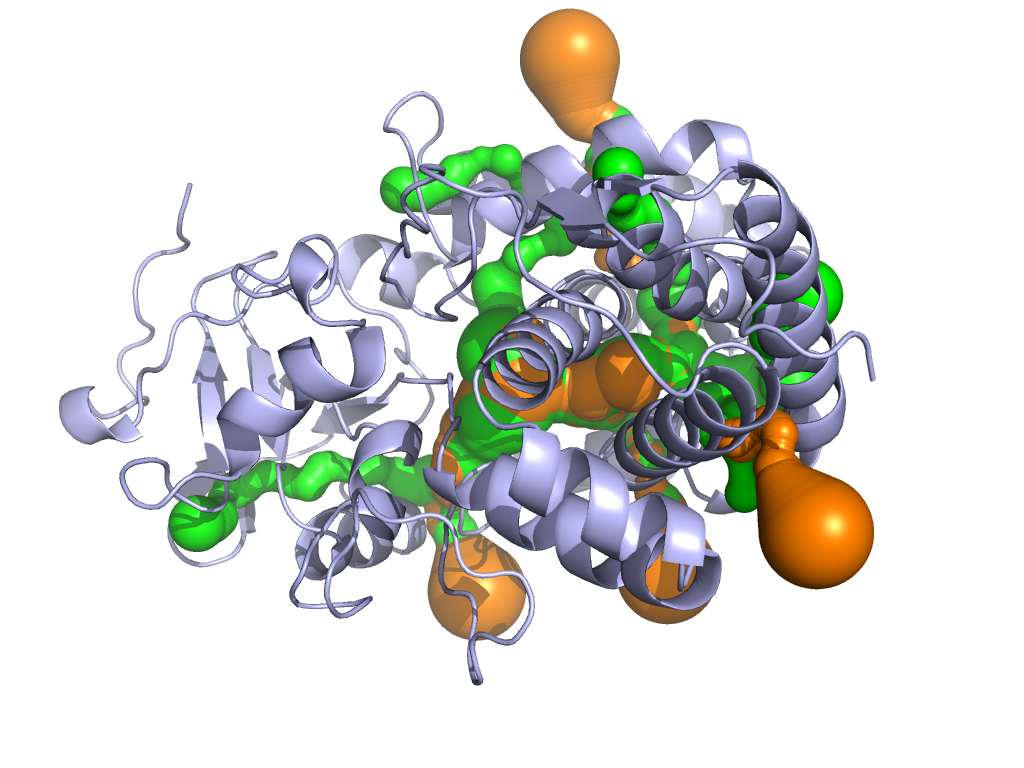
\includegraphics[width=0.22\textwidth]{fig/1akdprobe09-1} &
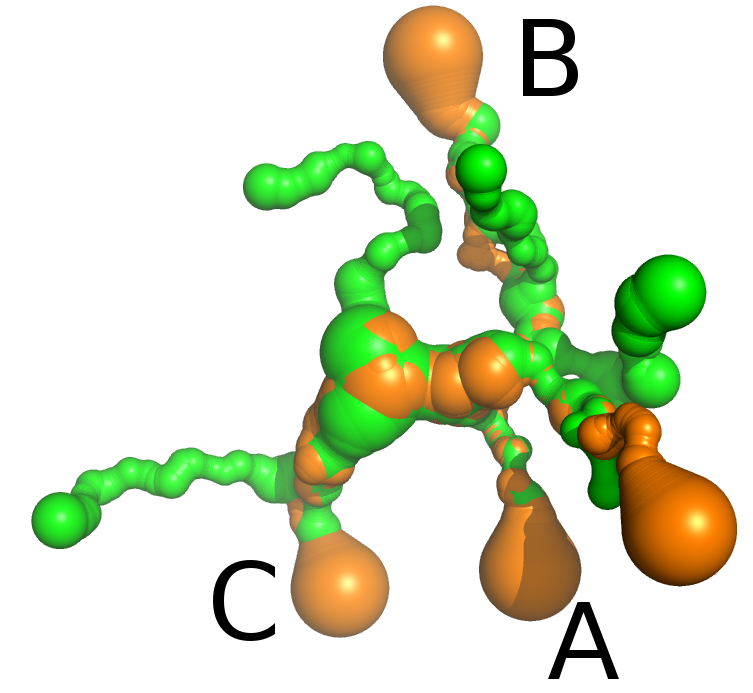
\includegraphics[width=0.18\textwidth]{fig/1akdprobe09-0-label} &
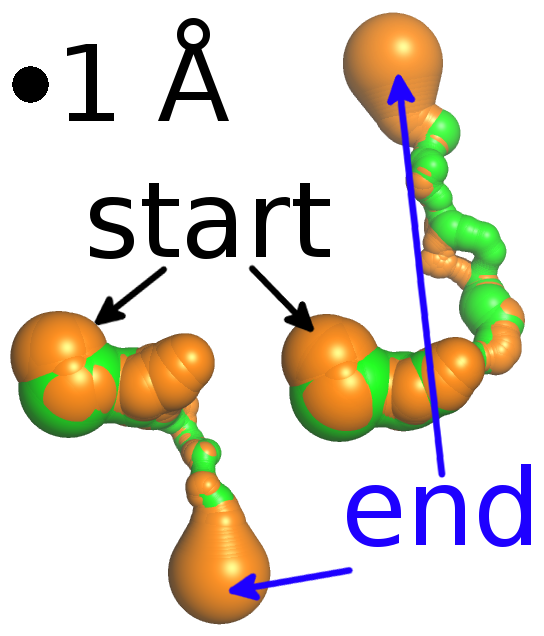
\includegraphics[width=0.12\textwidth]{fig/1akd-good} &
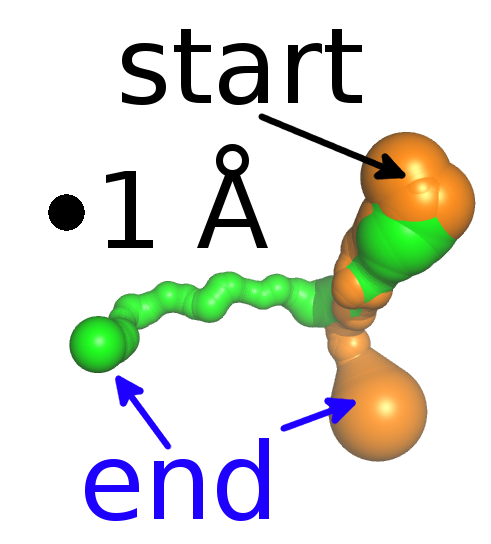
\includegraphics[width=0.105\textwidth]{fig/1akd-bad}  \\
(a) 1AKD tunnels      & (b) 1AKD tunnels only & (c) Correct tunnels (A,B)  & (d) Incorrect tunnels (C)
\end{tabular}
}
\caption{\label{fig::pic2}
    Tunnels detected in the protein 1AKD for $\probe=0.9$~\AA. 
Tunnels detected by \TA\ are depicted in orange, green spheres show tunnels computed by CAVER 3.0.
The protein with all tunnels detected by \TA\ method (a). 
The comparison between tunnels detected by \TA\ (orange) and CAVER 3.0 (green) (b) with highlighted three tunnels.
Examples of correctly detected tunnels --- green and orange spheres overlap in the most length of the tunnels (c).
Example of a CAVER tunnel (green) that has not been detected by \TA, as its nearest runnel (orange) does not overlap (d).
}
\end{figure*}




\begin{figure*}
\centering
{
\renewcommand{\arraystretch}{0.2}
%\renewcommand{\tabcolsep}{0pt}
\begin{tabular}{ccccc}
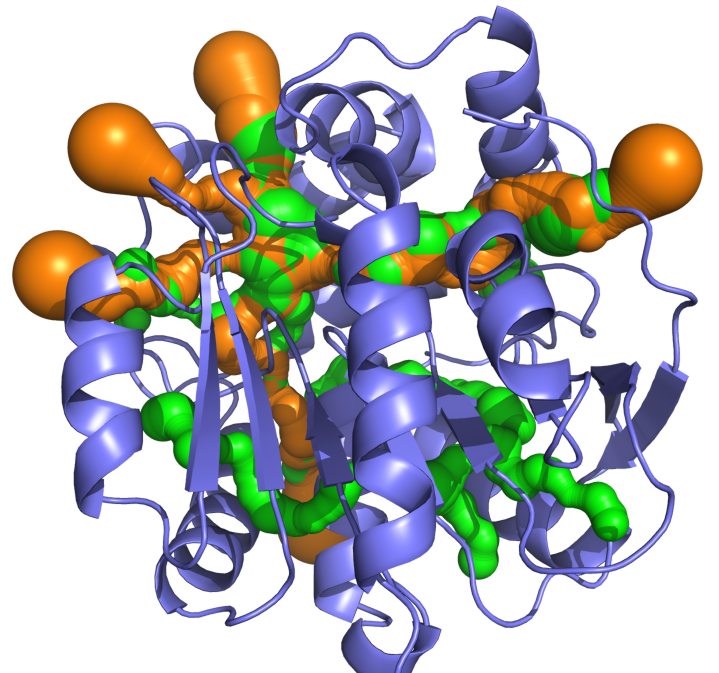
\includegraphics[width=0.22\textwidth]{fig/1cqw-main} &
%\includegraphics[width=0.3\textwidth]{fig/1cqw-caver} &
%\includegraphics[width=0.3\textwidth]{fig/1cqw-rrt} &
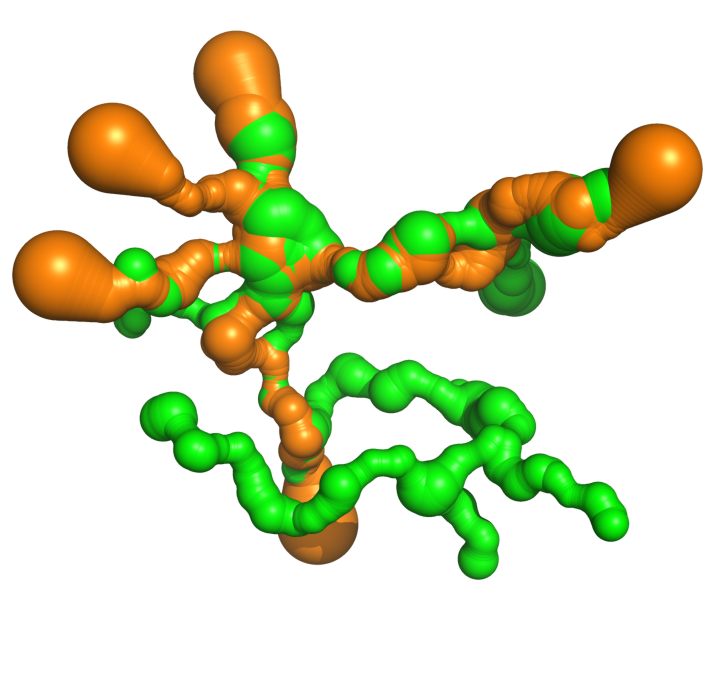
\includegraphics[width=0.22\textwidth]{fig/1cqw-tunnels} &
%\includegraphics[width=0.3\textwidth]{fig/1cqw-detailt2} \\
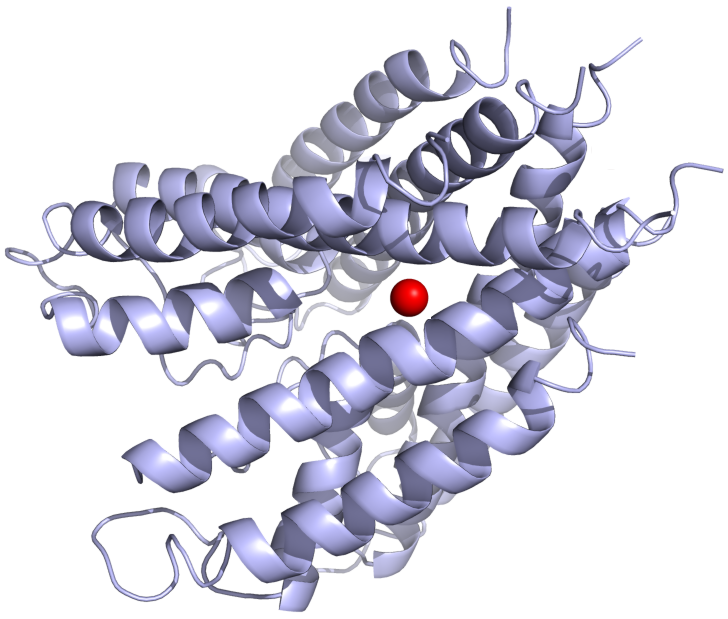
\includegraphics[width=0.23\textwidth]{fig/1bl8-center} &
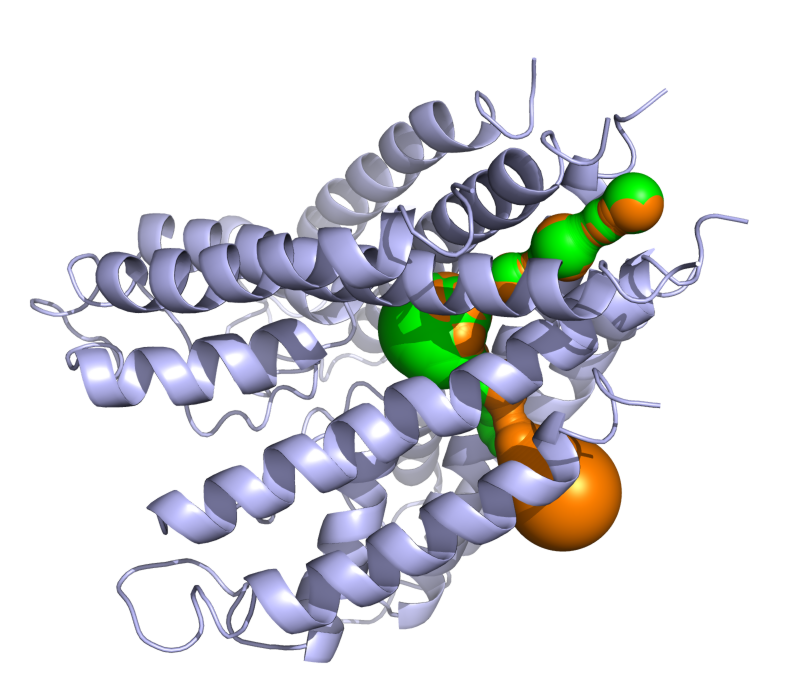
\includegraphics[width=0.23\textwidth]{fig/result1bl8-comp-09-1}  \\
%(a) Tunnels in 1CQW, probe $0.7$\AA & (b) 1CQW tunnels only & (c) Start positions in 1BL8 and 1BL8$^c$ & (d) Tunnel \#8 in 1BL8, probe 0.9~\AA
(a) Tunnels in 1CQW,      & (b) 1CQW tunnels only & (c) Start positions in  & (d) Tunnel \#8 in 1BL8, \\
probe 0.7~\AA            &                       & 1BL8        &     probe 0.9~\AA \\                                 
\end{tabular}
}
\caption{\label{fig::pic1}
Tunnels detected by \TA\ are depicted in orange, green spheres show tunnels computed by CAVER 3.0.
}
\end{figure*}



{\bf Tunnel detection in dynamic protein: }
A sequence of 1,000 frames of protein Haloalkane dehalogenase (DhaA) was analyzed with $\probe=0.9$.
Due to protein dynamics, the tunnels change rapidly and they often disappear or merge with others.
Each frame was analyzed with Alg.~\ref{alg::tunnel} with $\Imax=1000$ iterations.
Fig.~\ref{fig::dyn} shows visualization of selected frames.
In comparison to CAVER, that clusters the first tunnels found in each frame to a single 3D tunnel, the proposed
method can compute behavior or each detected tunnel separately.
Due to the CAVER's implicit clustering of the first tunnels, we do show any comparison of tunnels.
The total time to process the whole sequence was $\sim\!\!2$ minutes (@ 2.9 GHz), while CAVER took $\sim\!70$ minutes.
Due to space limits, only few images are shown in this section. 
We refer to \url{http://mrs.felk.cvut.cz/romoco2017} for more information.

\begin{figure*}
\centering
\begin{tabular}{cccc}
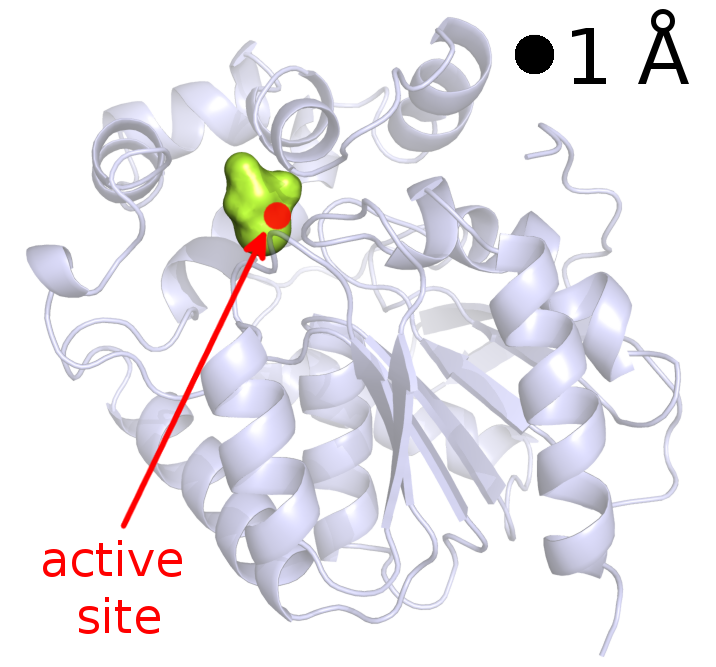
\includegraphics[width=0.2\textwidth]{fig/dcpmld2-6-label} &
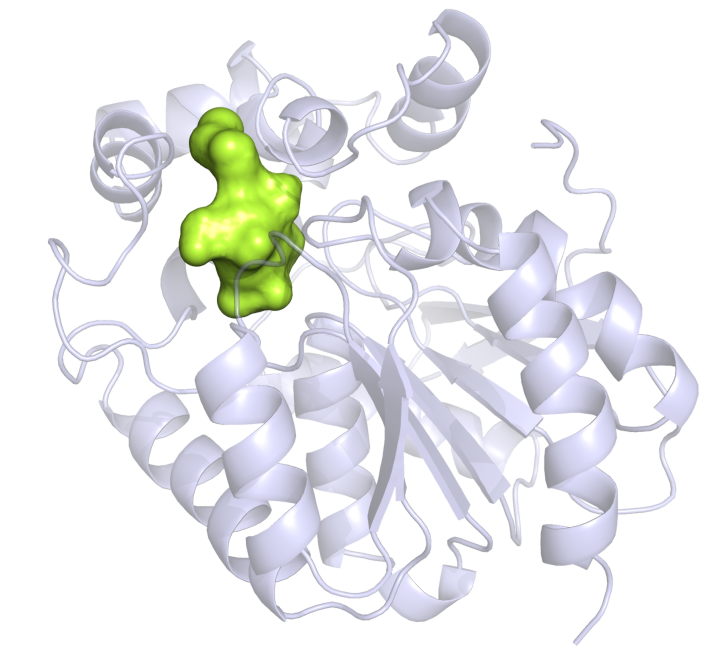
\includegraphics[width=0.2\textwidth]{fig/dcpmld2-12} &
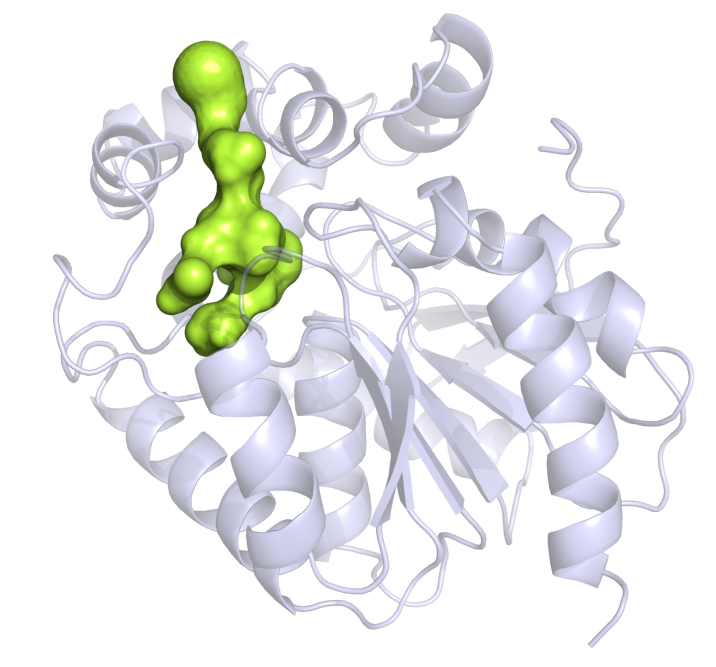
\includegraphics[width=0.2\textwidth]{fig/dcpmld2-19} &
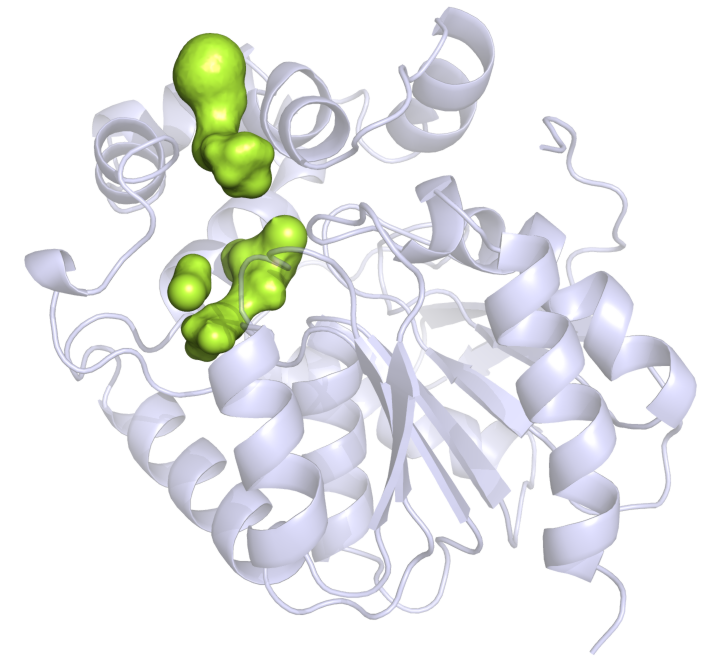
\includegraphics[width=0.2\textwidth]{fig/dcpmld2-20} \\
Frame 6 & Frame 12 & Frame 19 & Frame 20 \\                       
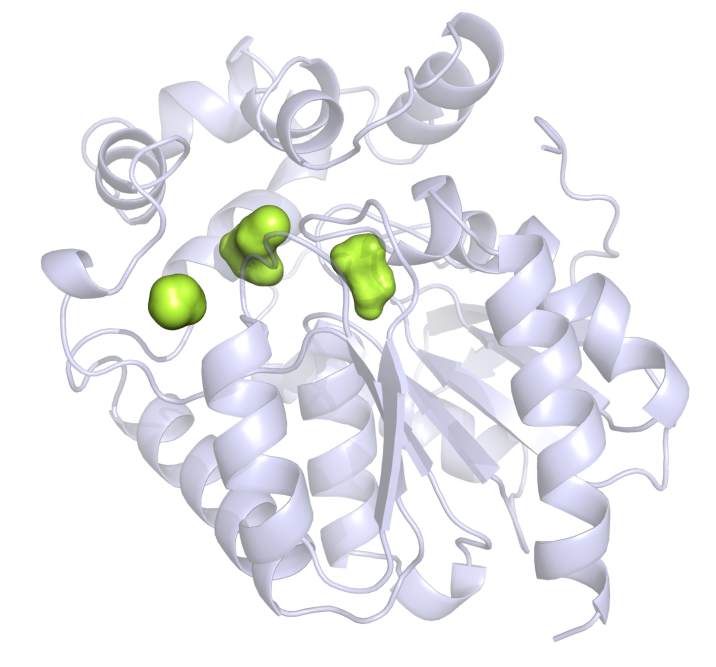
\includegraphics[width=0.2\textwidth]{fig/dcpmld2-48} &
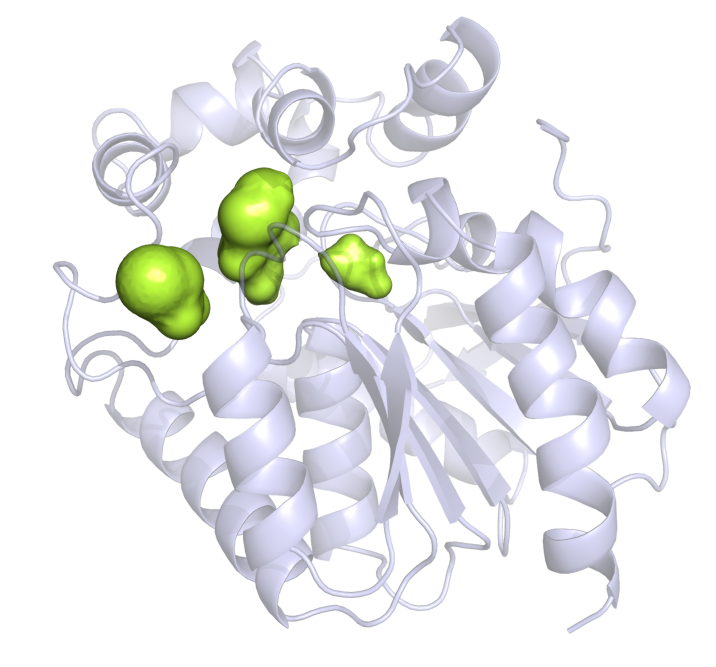
\includegraphics[width=0.2\textwidth]{fig/dcpmld2-54} &
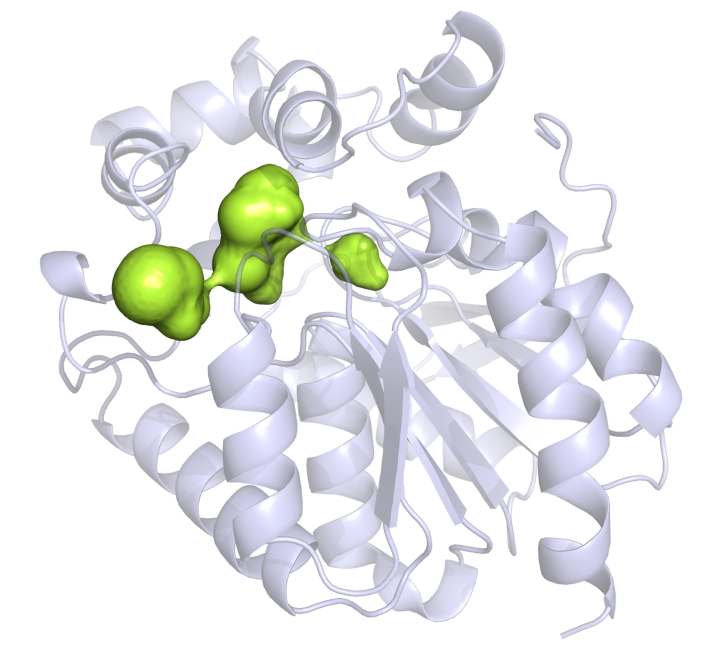
\includegraphics[width=0.2\textwidth]{fig/dcpmld2-55} &
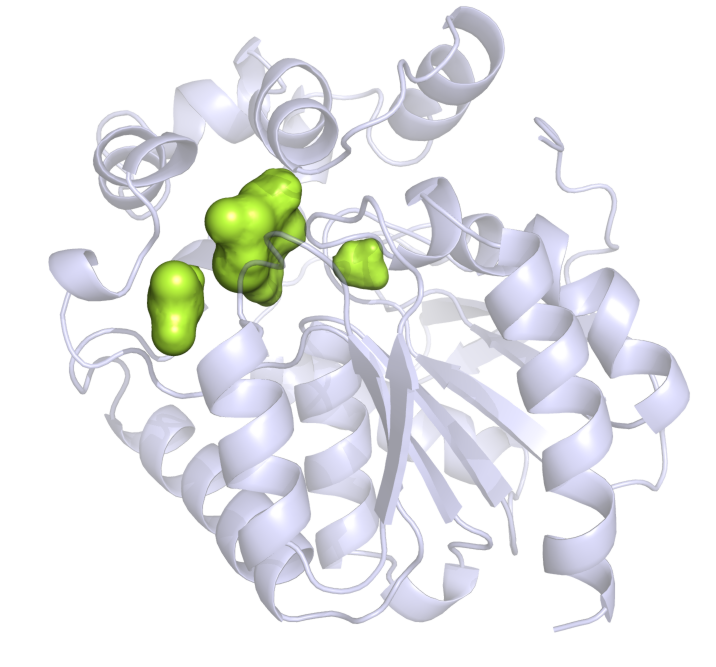
\includegraphics[width=0.2\textwidth]{fig/dcpmld2-56} \\
Frame 48 & Frame 54 & Frame 55 & Frame 56 \\                       
\end{tabular}
\caption{\label{fig::dyn}
Evolution of void space in molecular dynamics of the DHA protein. 
The active site is highlighted by the red circle in the top left image.
In the frame 20, the single tunnel is separated into three smaller tunnels.
Two of them temporarily connect in the frame 55, but then they remain unconnected.
}
\end{figure*}


\section{Conclusion }

The problem of tunnel detection in protein structures can be formulated as a path planning problem which can be solved by RRT.
%The paper shows how to utilize the RRT planner for this task.
%In comparison to existing techniques for tunnel detection, which are based on Voronoi Diagrams, the proposed method can find tunnels in a sequence of protein dynamics.
The tunnels have properties of narrow passages and it is therefore challenging to find path inside the protein.
We propose to generate random samples around a subset of Voronoi Diagram of the protein's atoms.
The subset is maintained automatically according to the distance to the configuration tree, so only the regions not reached yet
by the tree are sampled.
While the Voronoi diagram provides valuable information about suitable void regions in the protein, the
proposed RRT-based technique can cope with the protein dynamics.
The proposed technique can therefore be considered as an extension of the existing VD-based tools for tunnel detection.

\section{Acknowledgments}

The presented work has been supported by the Czech Science Foundation (GA{\v C}R) under research project No. 17-07690S.
Access to computing and storage facilities owned by parties and projects contributing to the National Grid Infrastructure MetaCentrum, provided under the programme "Projects of Large Infrastructure for Research, Development, and Innovations" (LM2010005), is greatly appreciated.


\bibliographystyle{plain}
\bibliography{paper}

\end{document}



